\documentclass[a4paper]{report}
\usepackage{setspace}
%\usepackage{subfigure}

\pagestyle{plain}
\usepackage{amssymb,graphicx,color}
\usepackage{amsfonts}
\usepackage{latexsym}
\usepackage{amsmath}
\usepackage{float}
\usepackage{rotating}
\usepackage[a4paper, margin = 3cm, bottom = 2.5cm]{geometry}
\usepackage{biblatex}
\addbibresource{bibliography.bib}

% Add autorefs with capitalized names (my preference)
\usepackage{hyperref}
\renewcommand{\chapterautorefname}{Chapter}
\renewcommand{\sectionautorefname}{Section}
\renewcommand{\subsectionautorefname}{Subsection}
\renewcommand{\subsubsectionautorefname}{Subsubsection}
\renewcommand{\figureautorefname}{Figure}
\renewcommand{\tableautorefname}{Table}

\newtheorem{theorem}{THEOREM}
\newtheorem{lemma}[theorem]{LEMMA}
\newtheorem{corollary}[theorem]{COROLLARY}
\newtheorem{proposition}[theorem]{PROPOSITION}
\newtheorem{remark}[theorem]{REMARK}
\newtheorem{definition}[theorem]{DEFINITION}
\newtheorem{fact}[theorem]{FACT}

\newtheorem{problem}[theorem]{PROBLEM}
\newtheorem{exercise}[theorem]{EXERCISE}
\def \set#1{\{#1\} }

\newenvironment{proof}{
PROOF:
\begin{quotation}}{
$\Box$ \end{quotation}}



\newcommand{\nats}{\mbox{\( \mathbb N \)}}
\newcommand{\rat}{\mbox{\(\mathbb Q\)}}
\newcommand{\rats}{\mbox{\(\mathbb Q\)}}
\newcommand{\reals}{\mbox{\(\mathbb R\)}}
\newcommand{\ints}{\mbox{\(\mathbb Z\)}}

%%%%%%%%%%%%%%%%%%%%%%%%%%


\title{{\vspace{-14em} 
\includegraphics[scale=0.4]{images/ucl_logo.png}}\\
{{\Huge AI Analyst: GenAI and financial data alert systems}}\\
}
\date{Submission date: 8 September 2025}
\author{Candidate Number: KYHL7\thanks{
{\bf Disclaimer:}
This report is submitted as part requirement for the MSc. Computer Science at UCL. It is substantially the result of my own work except where explicitly indicated in the text. The report may be freely copied and distributed provided the source is explicitly acknowledged.}
\\ \\
MSc. Computer Science\\ \\
Internal Supervisor: Prof. Lewis D. Griffin\\ \\
Repository: \url{https://github.com/davidve0206/ai-analyst}}



\begin{document}
 
\onehalfspacing

\maketitle


\tableofcontents

\setcounter{page}{1}
\begin{abstract}
This project set out to explore whether Large Language Model (LLM) driven agents can act as a junior data analyst in a corporate setting. The goal was to build a proof-of-concept “AI Analyst” that could access sales data, extract insights, and automatically generate reports on key performance indicators (KPIs). As such, the main challenge was to go beyond surface-level summaries and produce reports with the level of operational detail and causal reasoning that managers actually need, which are some of the weaknesses of LLMs.

The project combined research on agent architectures, orchestration frameworks, and evaluation methods with hands-on experimentation. Experiments were evaluated by a human judge guided by an explicit rubric, with reports graded on both \textit{form} and \textit{content}, alongside component-level automated evaluations and tests to ensure reliability.

Initial experiments using Microsoft’s Magentic-One architecture highlighted issues with context and task definition, leading to the development of a modular, workflow-driven system built in LangGraph. Thus, the project provided two outputs: first, the prototype which successfully delivered scheduled reports with relevant findings and operational insights, achieving all core requirements and demonstrating the feasibility of agentic AI for this use case; second, and perhaps more importantly, a set of key lessons from the development and experimentation process, which will be useful for the client's future work with Agentic AI systems.
\end{abstract}

\chapter{Introduction}
\label{chapter:introduction}

According to \cite{forrester2022}, by Forrester Consulting, knowledge workers spend 30\% of their time --- that is, 2.4 hours a day --- searching for information within their own company. This is not just critical due to time spent, but due to the impact on the business. As the same study puts it ``Teams are making poor or slow decisions based on the limited information in front of them, unaware of critical insights hiding in different tools". In the past, companies have invested on reducing time spent in this type of task by allowing teams to build their own apps and dashboards according to their needs. Still, building these dashboards takes resources, and executives still spend hours finding the exact information they need within those dashboard. In fact, this process is so complex, and yet so business critical, that companies sometime hire external advisors to support the creation and roll-out of these specialised tools. One of these external advisors is Alvarez \& Marsal (A\&M), a global professional services firm specialising in turnaround management, corporate restructuring, and performance improvement, who is the client for this project.

However, in recent years a radically new option has arisen. With the explosion of Large Language Models (LLMs), and subsequently of LLM-driven Agentic AI systems, a new family of task automation has become available, which allows the execution of complex, multi-step workflows autonomously. As such, the aim of this project is to explore the capabilities of AI Agents to act as a junior data analyst within a company, helping reduce the time spent by executives on finding the information they need.

The potential of AI Agents to perform this kind of data analysis is widely known. Agentic data retrieval, with tools like text-to-SQL agents, is already being widely explored in academia and starting to be adopted in industry, and there are benchmarks for LLM financial tasks such as stock price or earnings analysis. Still, there is still uncertainty about whether the quality and robustness that they could achieve in practice is actually at the level where such a system would be a benefit to a company. To gain a better understanding of this, the goal of this project is to create a proof-of-concept system, an ``AI Analyst", that can autonomously access a company's data, retrieve operational figures, extract initial insights from these figures and generate reports about a specific Key Performance Index (KPI) at set time intervals.

This specific use case poses a few challenges to the current state of the art in GenAI agents. For these reports, the AI Analyst must go beyond simply retrieving high-level data for the KPIs, it must also provide granular details that uncover deeper operational insights. For example, rather than merely reporting that sales are down by 10\%, the Analyst should also identify which products or regions are driving this decline.

This type of work is inherently open-ended. There is no single ``correct" answer, or even path to an answer, nor a clear point to stop, and the AI Analyst must adapt its approach depending on its own intermediate findings. Crucially, for the reports to be truly useful, the agent must not just report the data, but draw causal inferences that can point the manager in the right direction if any negative trend is found, something that remains a known challenge for LLMs, as shown by studies such as \cite{llmcausalreasoning2024}.

Moreover, this kind of internal analysis is not likely to be included in LLM's training sets because of confidentiality concerns. Companies rarely publish their internal data or reports, and certainly not the background of working notes that are preliminary to the final report. The closest likely data would be financial reports to investors, which might be available for public companies, but the requirements are different. Internal reports require more granularity, and usually include deep dives into specific operational findings.

A possible path to overcome these limitations would be to fine-tune a model on a company's internal data, such as their internal working notes and reports. Unfortunately this was not a possibility for this project as it would violate confidentiality clauses between A\&M and its clients. As such, the focus of the project remained on using Agentic AI systems with general purpose models.

This report is structured as follows. \autoref{chapter:research} reviews the state of the art in AI Agent orchestration, evaluation and prompting, along with the software tools available for building such systems. \autoref{chapter:requirements-analysis} outlines the process of defining project requirements in collaboration with Alvarez \& Marsal. \autoref{chapter:design-implementation} discusses the key implementation decisions, developed through a series of experiments with agent architectures and prompts. \autoref{chapter:evaluation-testing} describes the evaluation framework defined to assess these experiments. Finally, \autoref{chapter:reflections} reflects on the development of the proof-of-concept system, highlighting the main lessons learned and the potential future work towards a production-ready system.

\chapter{Research}
\label{chapter:research}

As this project takes a practical approach to exploring the capabilities of LLM-driven Agentic AI systems, its development was largely influenced by \cite{aiebook2025}, which ``provides a framework for adapting foundation models, which include both large language models (LLMs) and large multimodal models (LMMs), to specific applications". While this chapter does not intend to replicate the book's content, it will describe the most important learnings grasped from it, and add information from other relevant sources.

The chapter is divided in two sections. \autoref{sec:research-llms} details findings about the fundamental practical concepts for building Agentic AI applications. It describes what AI Agents and Agentic Systems are, the key concepts of prompt and context, and explores the complexities of evaluating this type of systems. \autoref{sec:research-tools}, on the other hand, describes the technology stack alternatives explored for building the agentic system, and its configuration frontend and scheduling execution of the AI Analyst.

\section{Large Language Models and Agents Learnings}
\label{sec:research-llms}

\subsection{Agent Architectures and Agentic Orchestration}

According to \cite{sapkota2025aiagentsvsagentic}, ``AI Agents can be defined as autonomous software entities engineered for goal-directed task execution within bounded digital environments'', usually with an LLM as their ``core reasoning component''. They distinguish AI Agents from Agentic AI, an ``emerging class of systems [that] extends the capabilities of traditional AI Agents by enabling multiple intelligent entities to collaboratively pursue goals through structured communication, shared memory, and dynamic role assignment''.

\subsubsection{Agent Architecture}

The basic structure of a single agent is described in \cite{aiebook2025} as an LLM which can perform certain actions in a defined environment through a set of defined tools. The LLM acts as the brain of this agent, processing the information it receives --- e.g., the task given by the user or results from its own tools --- and generating plans to perform the task. In this context, a plan can be imagined as a series of instructions to use the agent's tools.

The plans designed by the LLM can be performed in many ways. Tool calls can be executed in parallel or sequentially; the LLM and its requested tools can be called once, or in a loop until the LLM itself decides the task has been completed, etc. The design for how to perform this plan is generally called the agent's architecture.

One of the key problems for any Agent Architecture is introducing ways to adjust the initial plans laid out by the LLM, allowing them to correct potential errors. One of the most commonly used architectures is ReAct (Reasoning and Acting), proposed in \cite{yao2023react}. In this pattern, two steps are taken in a loop until the task is completed: a reasoning step, which encompasses both reflecting on tool outputs and creating or updating the plan, and an Action step, where the plan laid out in the reasoning step is executed --- that is, the tools are used according to the provided instructions.

This architecture was later expanded in \cite{shinn2023reflexion}, in their proposed Reflexion architecture. In this architecture, the agent has separate steps for (i) evaluating the output of its tools and (ii) self-reflecting on what went wrong or deeming the task as completed. On each loop, after the evaluation and reflection steps, the agent proposes a new plan, which is executed before returning to (i).

Most single-agent architectures follow one of these two general structures at their core, and the focus when developing individual agents is placed on defining the tools the agent can use and its prompts, which will be discussed in \autoref{sec:prompt-enginering}.

\subsubsection{Agentic Orchestration Architecture}

As described by \cite{sapkota2025aiagentsvsagentic}, Agentic AI systems are composed of multiple AI Agents that collaborate for more complex goals. Agentic orchestration thus refers to the way that the collaboration between agents is structured.

Some of the best-known ways to structure this collaboration, as described in \cite{langgraphagmultiagentsystems}, are networks (or swarms), where all agents communicate in a single group, and supervisor (or orchestrator) architectures, where an LLM acts as the coordinating node. However, agents can be coordinated in arbitrary ways depending on the needs of a specific task.

For instance, in \cite{fourney2024magenticone} a team of Microsoft researchers described Magentic-One, a generalist open-source system that demonstrated state-of-the-art performance in multiple agentic benchmarks. Their proposed architecture applies \cite{shinn2023reflexion}'s learnings to multi-agent orchestration by implementing ``a multi-agent architecture where a lead agent, the Orchestrator, plans, tracks progress, and re-plans to recover from errors". Moreover, according to \cite{fourney2024magenticone} ``Magentic-One's modular design allows agents to be added or removed from the team without additional prompt tuning or training, easing development and making it extensible to future scenarios''.

Due to its general capabilities, high performance in agentic benchmarks, ease of development and extensibility, the Magentic-One architecture was used extensively in this project.

\subsection{Prompt and Context Engineering}
\label{sec:prompt-enginering}

According to Chip Huyen in \cite{aiebook2025}, ``[a] prompt is an instruction given to a model to perform a task''. This instruction is usually split in a system (or developer) prompt and a user prompt. The system prompt contains general instructions that are relevant for any task that the LLM receives, it defines the way the LLM should approach the task, how tools are expected to be used, etc. The user prompt, on the other hand, describes the specific task that the LLM needs to perform. As described by \cite{wallace2024instructionhierarchytrainingllms}, some LLMs are post-trained to pay special attention to the system prompt.

Prompt engineering refers to the process of tweaking prompts to get the desired outcome from an LLM. This step is so important that model providers often provide detailed guides on how to write prompts for specific models, such as \cite{openai2025promptengineering} from OpenAI, which guided the prompt engineering process for this project.

Most of these guides, nonetheless, include two techniques that have become cornerstones for this process. First is ``few-shot'' prompting, introduced by \cite{brown2020languagemodelsfewshotlearners}, which demonstrated that language models can learn a desired behaviour from examples within the prompt. This technique is called as such in contrast to ``zero-shot'' prompts, which describe a task without providing any examples.

Second, there is ``Chain-of-Thought'' prompting, introduced by \cite{wei2023chainofthoughtpromptingelicitsreasoning}. In this type of prompt, the model is asked to perform a step-by-step process before providing an output --- the steps can be predefined in the prompt, or the model can be requested to define its own steps to follow during execution. Wei et al. were able to achieve state-of-the-art results using this technique.

Note that these techniques are not mutually exclusive, and prompts for complex tasks might include both of them, or none, depending on the needs of the task, how common it might be on the LLM's training data, and particularly the specific model used. For instance, some reasoning models might not need explicit chain-of-thought prompting.

\subsubsection{Context Engineering}

Borrowing \cite{aiebook2025}'s definition, the context is ``the information provided to the model so that it can perform a given task''. Context, thus, is all the information that is sent to the LLM when it is invoked, for example, the conversation history with the user, or background information included within the prompt. Context engineering is thus the process of tweaking what information is shared with the LLM to achieve the desired outcome.

One key pattern for context engineering is Retrieval Augmented Generation (RAG), which according to AI Engineering can be considered as ``a technique to construct context specific to each query". The pattern of retrieving and then generating was first introduced by Chen et al. in \cite{chen2017readingwikipediaansweropendomain}, where their system would retrieve Wikipedia pages relevant to a question and add their content to a model's context, and then fully coined as RAG, using vector indexing, by \cite{lewis2021retrievalaugmentedgeneration}.

While these two papers created the technique by adding text to the context, this pattern can be applied to any type of information, such as images or documents for multimodal models. Most relevant to this project, however, tabular data can also be retrieved and provided as part of the context.

But adding information is not the only way to manage a task's context. In perhaps the most important finding for this project, \cite{veseli2025positionalbiasesshiftinputs} demonstrates that as the size of the context grows closer to the model's limit, retrieval and reasoning become more biased towards data that is near the end of the context, and the model more easily fails to retrieve information provided in previous parts of the context. Thus, a key task of context engineering is limiting the size of the context while still providing all the information the LLM needs.

\subsection{LLM-Driven Systems Evaluation}
\label{sec:llm-evaluation}

Evaluation is a key aspect of developing any system, as it provides a way to control the quality of its outputs. However, this is particularly hard for LLM systems. \cite{aiebook2025} highlights two main reasons why: First, as tasks become more sophisticated, it takes more effort to evaluate them. As she puts it, ``[y]ou can no longer evaluate a response based on how it sounds. You'll also need to fact-check, reason, and even incorporate domain expertise". Second, the open-ended and probabilistic nature of LLMs ``undermines the traditional approach of evaluating a model against ground truths". There are too many potential correct responses, and thus it is impossible to have a comprehensive list of correct outputs as ground truths.

These problems are exacerbated when it comes to AI Agents, as they tackle more complex tasks. This is an ongoing research field but, according to \cite{krishnan2025aiagentsevolutionarchitecture}, the evaluation metrics so far are ``predominantly focused on accuracy metrics that measure task completion success". This focus has been criticised for many reasons, particularly for its narrow-sightedness. Limiting the evaluation to a task being completed or not ignores other important aspects of a system, such as its efficiency.

This type of measure is often called ``exact evaluation'' because it has no ambiguity --- a task is complete or it is not ---, and can be viewed more generally to include any type of rules-based evaluation. In rules-based evaluation, as the name indicates, a set of rules is defined, and the output is measured by its adherence to these rules. Despite the aforementioned narrow-sightedness, these types of evaluation are popular due to their ease of definition.

The alternatives to this type of evaluation are what has been called ``objective evaluations'', where an external validator reviews the agent's output and ``judges'' it, assigning it a score based on some type of defined criteria --- for example, completeness or clarity. So far, studies such as \cite{wang2025replacehumanevaluators} have found that this judgment can be performed by either LLMs (called LLM as a judge) or Humans (called Human as a judge), with high correlations in the scores given. Although \cite{hu2023decipher} found that personal preferences can affect the score a human evaluator gives to an output, which might prove there is an advantage to using LLMs.

Still, these approaches rely solely on the final output for evaluation, something that is criticised by other studies, such as \cite{zhuge2024agentasajudgeevaluateagentsagents}. They believe that agents shouldn't only be evaluated on their final output but on the intermediate steps taken, and thus propose agent as a judge, a methodology that uses agents to extract and evaluate intermediate outputs, as a better alternative.

Despite the lack of a clear ``best" strategy, evaluation is one of the most important parts of developing an Agentic AI system. \cite{aiebook2025} goes as far as proposing a development methodology called Evaluation Driven Design (EDD) which, similarly to Test Driven Design, defines the evaluation criteria for the application before building the application, allowing safe iterations from the beginning. But how do you define these evaluation criteria? Huyen proposes thinking in three categories for evaluating LLMs, which can be adapted as follows for Agentic systems:

\begin{itemize}
    \item Domain-specific capacity: Evaluating the ability of the agent to perform tasks specific to the problem domain, such as coding or finance.
    \item Generation capacity: Evaluating the quality of the text being generated, such as its factual consistency.
    \item Instruction-following capacity: Evaluating how well the specific instructions of a prompt are followed.
\end{itemize}

\subsubsection{Choosing the Right Model}

The difficulty in evaluation of LLMs and Agents highlights a key challenge: choosing the right model, or models, to power the agent. In theory, the best way to decide which models to use would be to evaluate the system with different models, but this adds complexity in how the system must be built --- different models can have different APIs, work better with different prompt structures, etc. In practice, thus, models are usually selected before developing the system, either through narrow evaluations, benchmarks or a project's specific needs.

For example, if compute efficiency is a key need, the literature regarding model selection suggests using specialised models for tasks that require domain-specific capabilities, such as data analysis, and more general models for tasks that are common in the general training data, such as coding, tool calling or general summarisation (e.g., writing the final report). For the use case of this project, studies such as \cite{ke2025demystifyingdomainadaptiveposttrainingfinancial} and \cite{tanabe2024enhancingfinancialdomainadaptation} have shown that smaller models specifically trained for financial tasks outperform larger models in financial benchmarks.

Nevertheless, \cite{lu2025bizfinbench} created a financial benchmark that includes finance-specific tasks such as forecasting market trends, predicting asset movements, or analysing causal relationships in financial events, which closely resemble the types of tasks required in this project. Their evaluations of general models such as OpenAI's GPT-4o or o4-mini produced some of the highest results in their sample --- above 80\% --- for these tasks. While these are less efficient, they are more easily available and thus can be a good choice for a proof of concept.

\section{Software Tools}
\label{sec:research-tools}

While the project involved numerous decisions about tools, such as libraries to use for certain functionalities, this section will only detail the research performed to make the key decisions to build the system: the frameworks that could be used for user interface and agent orchestration, and the potential tools to schedule agent runs. These will be presented in order of importance.

An important note is that the client had a preference for using Azure/Microsoft products for any infrastructure requirements, due to their enterprise readiness. Azure was thus used as inference provider (i.e., LLMs calls are performed through Azure AI Foundry). The client could not provide access to their own instances though, so the Azure student subscription was used, though it came with limitations in model access and rate limiting. They also preferred to use Python as the development language, thus no alternative language was explored.

\subsection{Agent Orchestration Frameworks}

Selecting the appropriate orchestration framework was the most impactful stack decision for the project. As the list of options is extensive, the first criteria to narrow it down was the size of a framework's community, which is often indicated by the number of GitHub stars of its repository. Community size can significantly influence the availability of resources such as documentation, tutorials, and general support. A larger community typically leads to more comprehensive examples and a broader base of shared knowledge, facilitating smoother development and troubleshooting.

As such, \autoref{tab:orchestration_frameworks_stars} compares several prominent Python frameworks for agentic orchestration, highlighting their community size and the implications in terms of support and resources, while \autoref{tab:orchestration_frameworks_uses} summarizes findings on the same frameworks' functionality, ideal use cases, and the pros and cons associated with each.

\begin{table}[h]
\centering
\begin{tabular}{|p{3cm}|p{2.5cm}|p{8.2cm}|}
    \hline
    \textbf{Framework} & \textbf{GitHub Stars} & \textbf{Support and Resources Notes} \\ \hline
    \textbf{LangChain and \newline LangGraph} & 113.6k \newline (LangChain) & Actively maintained open-source framework. Extensive tutorials, active forums, and a wide array of integrations. \\ \hline
    \textbf{LlamaIndex} & 44k & Well-maintained open-source framework. Good documentation, data-centric, growing ecosystem including LlamaHub, Discord, and examples. \\ \hline
    \textbf{AutoGen} & 43.1k & Used to have support from Microsoft, with growing number of examples, but currently in the process of being merged to Semantic Kernel. \\ \hline
    \textbf{CrewAI} & 35.8k & Active development. Fewer community resources than LangChain but more than Microsoft's frameworks. \\ \hline
    \textbf{Semantic Kernel} & 25.8k & Backed by Microsoft, in active development. Documentation and community resources focused on C\#. \\ \hline
\end{tabular}
\caption{Comparison of Python Agentic Orchestration Frameworks}
\label{tab:orchestration_frameworks_stars}
\end{table}


\begin{table}[h]
\centering
\begin{tabular}{|p{3cm}|p{3cm}|p{2.5cm}|p{5.5cm}|}
    \hline
    \textbf{Framework} & \textbf{Functionality} & \textbf{Use Cases} & \textbf{Pros and Cons} \\ \hline
    \textbf{LangChain and \newline LangGraph} & Modular pipeline for LLMs, embeddings, tools & Complex workflows, data pipelines & Pros: Extensive integrations, strong community support \newline Cons: Steep learning curve, large framework size \\ \hline
    \textbf{LlamaIndex} & Data-centric framework for indexing, retrieval, and RAG. & Chatbots, retrieval systems, knowledge-base querying & Pros: Excellent data ingestion and RAG strategies, good documentation \newline Cons: Smaller community than LangChain, implementation tightly coupled to data source \\ \hline
    \textbf{AutoGen} & Multi-agent orchestration with conversational agents & Multi-agent systems, collaborative tasks & Pros: Easy to implement multi-agent system, original implementation of Magentic-One \newline Cons: In the process of deprecation in favour of Semantic Kernel \\
    \hline
    \textbf{CrewAI} & Role-based collaboration with task management & Team-based workflows, sequential tasks & Pros: Intuitive design, good for structured workflows \newline Cons: Less flexibility for complex scenarios, smaller community \\
    \hline
    \textbf{Semantic Kernel} & Enterprise-grade framework & Enterprise applications, integration with Microsoft tools & Pros: Strong enterprise support, robust features, includes a default implementation of Magentic-One \newline Cons: Limited Python support, smaller community \\
    \hline
\end{tabular}
\caption{Comparison of Python Agentic Orchestration Frameworks}
\label{tab:orchestration_frameworks_uses}
\end{table}

As will be explained in more detail later, the development of the project consisted of two stages. The first stage tried to take advantage of Microsoft's Magentic-One orchestration architecture, and that, in combination with the use of Azure as inference provider, made it an easy choice to use Semantic Kernel. On the contrary, the second stage's approach was to build a detailed workflow with careful management of the data used in each step's context, thus making LangChain/LangGraph a better fit in functionality. Moreover, the amount of documentation and community resources available could provide additional support in building this more detailed workflow. LangChain also has its own observability platform (LangSmith), which was used in this stage as it integrates easily with the framework.

\subsection{Scheduling Tool}

The project requires the AI agent to run at set intervals, defined by the user. As such, two scheduling alternatives were considered: Celery and cron (through the \texttt{python-crontab} library).

Celery is a distributed task queue that supports asynchronous and real-time task execution, with advanced features such as retries, task prioritisation, and integration with message brokers like Redis or RabbitMQ. While powerful, Celery introduces additional system complexity and overhead, requiring configuration of worker processes and a message broker.

In contrast, cron is a native, time-based scheduler available on Unix-like systems, designed specifically for executing tasks at fixed intervals. Cron is straightforward to configure, persistent across system reboots, and does not require any additional services.

Given the project's scope as a proof-of-concept, and the fact that the requirement was only periodic execution at set intervals, cron was selected as the more practical solution.

\subsection{User Interface Framework}

Finally, several Python frontend options were considered for the configuration interface. As shown in \autoref{tab:framework_comparison}, the main alternatives evaluated were Streamlit, Gradio, and FastAPI with Jinja2 templates. While Streamlit and Gradio offer very quick setup and ease of use for prototypes, FastAPI with Jinja2 was chosen for this project due to its high customisability and the ability to easily scale the proof-of-concept into a full production application if needed.

\begin{table}[h]
\centering
\begin{tabular}{|p{2.5cm}|p{4cm}|p{4cm}|p{4cm}|}
\hline
\textbf{Feature \rule{0pt}{0.5cm}} & 
\textbf{Streamlit \rule{0pt}{0.5cm}} & 
\textbf{Gradio \rule{0pt}{0.5cm}} & 
\textbf{FastAPI + Jinja2 \rule{0pt}{0.5cm}} \\ \hline
\textbf{Primary Use Case} & Interactive dashboards & ML model interfaces & API-driven web apps \\ \hline
\textbf{Ease of Setup} & Very easy; minimal code & Very easy; minimal code & Moderate; requires setup \\ \hline
\textbf{Customization} & Limited UI customization & Limited UI customization & High; full control \\ \hline
\textbf{Performance} & Moderate & Moderate & High; asynchronous support \\ \hline
\textbf{Extensibility} & Limited & Limited & High; supports plugins \\ \hline
\textbf{Recommended Deployment} & Streamlit Cloud & Gradio Hub & Flexible (e.g., Docker, Cloud) \\ \hline
\textbf{Best For} & Rapid prototyping & Quick ML demos & Scalable, production-ready apps \\ \hline
\end{tabular}
\caption{Comparison of Python Frontend Frameworks for AI Agent Configuration}
\label{tab:framework_comparison}
\end{table}

\chapter{Requirements and Analysis}
\label{chapter:requirements-analysis}

As mentioned before, the client for this project is Alvarez \& Marsal (A\&M), a global professional services firm specialising in turnaround management, corporate restructuring, and performance improvement.

A\&M clearly identified a problem. Even with the specialised tools they build for companies, executives spend valuable time navigating dashboards just to find the information that is relevant to their specific needs. As such, they wanted to explore the capabilities of AI Agents to reduce this time by building an Agentic AI system that can autonomously access a company's data, retrieve operational figures, extract initial insights from these figures and generate a report about a specific Key Performance Index (KPI), at set time intervals, based on the company's data.

Nevertheless, as a professional services firm, Alvarez \& Marsal had restrictions on the resources they could share for the development of the system, particularly, due to client confidentiality clauses. As such, the requirement elicitation process was performed through a series of meetings with A\&M where they provided context on the needs of their clients and shared bullet points with thoughts on potential functionalities for the system.

Considering the limitations caused by client confidentiality clauses, it was agreed to build an exploratory proof-of-concept system that could provide key insights about the problem, and later be extended by A\&M's team. This chapter details the process for arriving to the requirements for this proof-of-concept system. First, it describes the creation of user personas, and their scenarios for using the system, which helped envision the key need for final users. Second, it describes the process of defining and prioritising the system's requirements based on said personas and A\&M's inputs. Finally, it notes a byproduct of this process, the definition of the structure of the report that the agent should generate.

\section{User Personas and Scenarios}

Based on their experience advising companies, A\&M identified 2 types of users that could reap the highest benefits from this type of system: Sales Managers and a Chief Financial Officers (CFOs). Following the design thinking methodology, drawing heavily from the Interaction Design Foundation's advice in \cite{ixdf_personas_2025} and \cite{ixdf_user_scenarios_2025}, it was decided to create user personas for each of these types of user to better understand a potential user's needs and goals.

Due to the same confidentiality reasons mentioned before, this could not be done through user research. Instead, the following are fictional personas created based on both on A\&M and the author's experience in industry.

\subsubsection{John, the Sales Manager}

\begin{tabular}{|p{3.3cm}|p{10.5cm}|}
\hline
\textbf{Hard Facts} & John lives in London, is 30--35 years old, and works as the Sales Manager for Germany for a car parts manufacturer. \\
\hline
\textbf{Computer and Internet Use} & He mainly uses a computer for work: sending and receiving emails, reviewing dashboards, and browsing the internet for news and social media. He also owns an iPad and a MacBook. He is comfortable with computers but isn't particularly tech-savvy. \\
\hline
\textbf{A Typical Monday} & John starts his work week by reviewing unread emails to set priorities. He can spend up to two hours reviewing the company's dashboard to track sales in Germany. After these two hours he schedules follow-up meetings, either with his team or clients. He spends the rest of his day in said meetings. \\
\hline
\textbf{Current Scenarios (As is)} & 
\begin{minipage}[t]{\linewidth}
    \begin{itemize}
        \item \textbf{All good}: John navigates a dashboard to see that sales are on track with expectations, he then moves on with his day.
        \item \textbf{Issue found}: John notices a sales decline and spends a few hours investigating by manually filtering through different dashboard views (sales per client, number of active clients, sales by product). He notes a reduction in total clients, and thus requires his team to investigate what clients churned and why. He then works with his team to create an action plan based on their findings.
        \item \textbf{Continue what's working}: John sees a better-than-expected sales increase, and spends an hour investigating by looking at top clients and specific products. He decides to look for news and finds an article about a change in safety regulations that might be driving the trend. He then advises his team to review the regulation and try to upsell more customers.
    \end{itemize}
    \vspace{0.05em}
\end{minipage} \\
\hline
\textbf{Future Scenarios (To be)} & 
\begin{minipage}[t]{\linewidth}
    \begin{itemize}
        \item \textbf{All good}: John receives an email with a short report showing sales are on target, skims it, and moves on with his day.
        \item \textbf{Issue found}: John receives an email with a report attached that notes a sales decline and lists the clients who have churned and their commonalities, allowing him to forward the report to his team and schedule a meeting to discuss.
        \item \textbf{Continue what's working}: John receives an email with a report pointing out a higher-than-expected increase in sales for a specific product and links to a news article about a change in safety regulations. He can forward the report and advise his team based on the news.
    \end{itemize}
    \vspace{0.05em}
\end{minipage} \\
\hline
\end{tabular}


\subsubsection{Clara, the CFO}

\begin{tabular}{|p{3.3cm}|p{10.5cm}|}
\hline
\textbf{Hard Facts} & Clara lives in Cambridge with her family, is 45--50 years old, and works as the CFO of John's company. \\
\hline
\textbf{Computer and Internet Use} & She mainly uses a computer for work: sending and receiving emails, reviewing dashboards, and browsing the internet. She is definitely not a tech-savvy person. \\
\hline
\textbf{A Typical Monday} & Clara starts her week by reviewing emails and spends up to an hour reviewing the company's dashboard to identify high-level trends. She has lunch with the CEO to discuss strategic planning and spends the afternoon in meetings with her team. \\
\hline
\textbf{Current Scenarios (As is)} & 
\begin{minipage}[t]{\linewidth}
    \begin{itemize}
        \item \textbf{All good}: Clara navigates through different dashboard screens to check various KPIs and finds they are all on track. She then moves on with her day.
        \item \textbf{Issue found}: Clara notices a decline in Gross Margin, and spends a few hours investigating by manually filtering her sales dashboard and cost dashboard for clues. She finds an unexpected cost increase in France and instructs her team to investigate further.
        \item \textbf{Continue what's working}: Clara sees an increase in sales growth, and spends a few hours investigating by filtering her sales dashboard by business lines, countries, etc. She finds the increase is driven by the Brakes division, and by the Germany unit. She then looks for news, finds a regulation change in Germany, and schedules a meeting with the corresponding sales team to strategise how to replicate this in other countries.
    \end{itemize}
    \vspace{0.05em}
\end{minipage} \\
\hline
\textbf{Future Scenarios (To be)} & 
\begin{minipage}[t]{\linewidth}
    \begin{itemize}
        \item \textbf{All good}: Clara receives an email with a short report on all the KPIs she monitors, skims it, and moves on with her day.
        \item \textbf{Issue found}: Clara receives an email with a report mentioning the Gross Margin decline, as well as a detailed explanation of the cause --- increased costs in the France unit. She forwards the report to her team and instructs them to investigate further.
        \item \textbf{Continue what's working}: Clara receives an email with a report that points out an increase in sales growth, driven by the Brakes product group in Germany. The report also links to a news article about a potentially related safety regulation change. This allows her to schedule a meeting with the corresponding sales team to discuss the impact and prepare for similar changes in other countries.
    \end{itemize}
    \vspace{0.05em}
\end{minipage} \\
\hline
\end{tabular}

\subsection{Analysis}

As put in \cite{ixdf_personas_2025}, Fictional Personas are deeply flawed, but they can be used as initial sketches of user needs. For this project, these two user personas highlighted a few things that would be important to drive adoption of any proposed solution:

\begin{enumerate}
    \item \textbf{The user interface should be easy to use:}
    \begin{itemize}
        \item Target personas are not particularly tech-savvy.
        \item They are used to the intuitive interface of dashboards.
        \item They don’t want to spend 5 hours setting something up that saves them a few hours, they want to spend 5 minutes.
        \item Their primary need is direction on where to look more closely for their next steps, or instruct their team to do so, meaning a high-level report can be adequate for early adopters.
    \end{itemize}

    \item \textbf{Different users target a different number of KPIs, and this affects the level of detail they want to see:}
    \begin{itemize}
        \item A Sales Manager tracks a single KPI (Sales), but they want to understand the operational detail. A CFO, on the other side, follows multiple high-level KPIs, but only wants to have a general grasp of the situation.
        \item The current solution might be less efficient, but allows them to see exactly the level of operational detail they want. The system must be aware of that level of detail and replicate that feeling.
    \end{itemize}

    \item \textbf{Users want a quick way of knowing if they need to review the report in detail:}
    \begin{itemize}
        \item The report must contain an Executive Summary that provides a quick glance to its contents.
        \item The report must clearly state any ``special case" present. ``Special cases" includes negative performance in KPIs, such as a reduction in margin, or changes in trends.
        \item The body of the email that delivers the report should also include the key findings.
    \end{itemize}
\end{enumerate}

\section{MoSCoW Requirements}

% Define counters
\newcounter{frcounter}
\newcounter{nfrcounter}

% Formatting for IDs
\newcommand{\frid}{FR-\arabic{frcounter}}
\newcommand{\nfrid}{NFR-\arabic{nfrcounter}}

The base of the requirements listed below was the list of potential functionalities provided by A\&M at the beginning of the project. This initial set of high-level requirements was then made concrete and prioritised using the MoSCoW method, guided by insights from the user perrsona analysis process and A\&M's confidentiality needs.

The analysis of user personas not only helped understand what functionalities would be more important for actual users, but highlighted the differences between the needs of the two types of users. In practical terms, it made it clear that the level of detail of the reports for the two types of personas are different, and thus the prompts used for one type of user might not work for the other. As such, it was decided to split certain requirements related to the report content by type of user.

Additionally, as mentioned earlier it was agreed with A\&M that the system created would be an exploratory proof-of-concept, as client confidentiality clauses restricted the data that they could share. This restricted the possibility of implementing some requirements. A key example was using online information sources, the system would not be able to identify if news are relevant when using anonymised data, thus it wouldn't make sense to implement in this stage.

However, knowing what requirements might be implemented in the future can inform decisions in the present. As such, it was deemed acceptable to have a long list of Won't Have requirements --- that is, a long list of requirements that are known and wanted for the system, but that will be outside of the scope of this project.

Finally, due to the limitations on data availability, it was decided that the proof-of-concept would only cover Sales Manager users. While A\&M could anonymise sales data with relative speed \footnote{This speed came with a cost. As you can notice in the sample report provided in the appendix, there are some drastic fluctuations in sales that can only be explained by data lost while anonymising.}, the time needed to anonymise enough data for other KPIs was deemed too long for the needs of the project.

\subsection{Functional Requirements}

\subsubsection{Sales Manager}

\begin{tabular}{|l|p{10cm}|l|}
\hline
\textbf{ID} & \textbf{Requirement} & \textbf{Priority} \\
\hline
\stepcounter{frcounter}\frid & The system shall allow a Sales Manager-type user to set up a scope for their report (e.g., a specific region or product) & Must Have \\ \hline
\stepcounter{frcounter}\frid & The system shall be able to generate a report based on the user’s preferences & Must Have \\ \hline
\stepcounter{frcounter}\frid & The system shall be able to identify “special cases” in Sales trends and perform a deeper analysis & Must Have \\ \hline
\stepcounter{frcounter}\frid & The system shall be able to provide a simple Sales forecast based on current trends & Should Have \\ \hline
\stepcounter{frcounter}\frid & The system shall be able to recommend potential actions to remedy “special cases” in Sales trends & Should Have \\ \hline
\stepcounter{frcounter}\frid & The system shall be able to provide simple Sales forecasts based on the remedy actions recommended by itself & Could Have \\ \hline
\stepcounter{frcounter}\frid & The system shall be able to provide advanced Sales forecasts using regression techniques or any other statistical method & Won’t Have \\
\hline
\end{tabular}

\subsubsection{CFO}

\begin{tabular}{|l|p{10cm}|l|}
\hline
\textbf{ID} & \textbf{Requirement} & \textbf{Priority} \\
\hline
\stepcounter{frcounter}\frid & The system shall allow a CFO-type user to set up a list of KPIs they want their report to follow & Won’t Have \\ \hline
\stepcounter{frcounter}\frid & The system shall be able to generate a report for the user’s KPI list & Won’t Have \\ \hline
\stepcounter{frcounter}\frid & The system shall be able to provide simple forecasts for each KPI based on current trends & Won’t Have \\ \hline
\stepcounter{frcounter}\frid & The system shall be able to identify “special cases” in the trend of any KPI and perform a deeper analysis & Won’t Have \\ \hline
\stepcounter{frcounter}\frid & The system shall be able to recommend potential actions to remedy “special cases” in each KPI’s trend & Won’t Have \\ \hline
\stepcounter{frcounter}\frid & The system shall be able to provide simple forecasts for each KPI based on the remedy actions recommended by itself & Won’t Have \\ \hline
\stepcounter{frcounter}\frid & The system shall be able to provide advanced forecasts for each KPI using regression techniques or any other statistical method & Won’t Have \\
\hline
\end{tabular}

\subsubsection{User Type Independent Requirements}

\begin{tabular}{|l|p{10cm}|l|}
\hline
\textbf{ID} & \textbf{Requirement} & \textbf{Priority} \\
\hline
\stepcounter{frcounter}\frid & The system shall email the resulting report to the email addresses configured by the user & Must Have \\ \hline
\stepcounter{frcounter}\frid & The system shall include both financial and operational information in a report & Must Have \\ \hline
\stepcounter{frcounter}\frid & The system shall be able to load information from a CSV file & Must Have \\ \hline
\stepcounter{frcounter}\frid & The system shall customise the email body with the key findings of the report & Should Have \\ \hline
\stepcounter{frcounter}\frid & The system shall be able to load information from other files provided by the user & Won't Have \\ \hline
\stepcounter{frcounter}\frid & The system shall be able to load information from a set of reliable online information sources & Won't Have \\ \hline
\end{tabular}

\subsection{Non-Functional Requirements}

\begin{tabular}{|l|p{10cm}|l|}
\hline
\textbf{ID} & \textbf{Requirement} & \textbf{Priority} \\
\hline
\stepcounter{nfrcounter}\nfrid & The system shall be extensible to other sources of information & Must Have \\ \hline
\stepcounter{nfrcounter}\nfrid & The system shall run autonomously at fixed intervals & Must Have \\ \hline
\stepcounter{nfrcounter}\nfrid & The system shall allow the user to update the fixed interval at which it runs & Must Have \\ \hline
\stepcounter{nfrcounter}\nfrid & The system shall provide a user interface to update its configuration & Should Have \\ \hline
\stepcounter{nfrcounter}\nfrid & The system shall provide a user interface that is clear and easy to use & Should Have \\ \hline
\stepcounter{nfrcounter}\nfrid & The system shall allow multiple users to set up their reports & Could Have \\ \hline
\stepcounter{nfrcounter}\nfrid & The system shall allow users to authenticate before updating their report preferences & Won’t Have \\ \hline
\end{tabular}

\section{Report Structure}

A byproduct from the requirement elicitation process was the structure of the report that the agent should generate. This is not considered part of the system's requirements, as the structure of the report can and should change over time as functionality is added to the system, but an initial structure based on the Must Have and Should Have requirements was agreed with Alvarez \& Marsal during this process:

\begin{enumerate}
    \item Executive Summary: A quick glance of the key findings.
    \item Overview: An overview of the value of the KPI for the period.
    \item Trends and Context: An overview of the trend for the KPI and high-level operational metrics.
    \item In depth analysis: A detailed analysis of operational metrics that drive the trend.
    \item Forward Outlook and Recommendations: A projection of the KPI and potential ways to correct negative trends.
\end{enumerate}

\chapter{Design and Implementation}
\label{chapter:design-implementation}

As an exploratory proof-of-concept, the project's system exactly as built will likely never be used in a production environment. In fact, at the time of writing it is not deployed anywhere. Nevertheless, its implementation followed two guiding principles that should make it easy for the client to either build upon it or take useful parts for their production system: \textit{modularity} and \textit{extensibility}.

These principles were followed not only in the high-level design, explained in \autoref{sec:system-design}, but in the detailed implementation, detailed in \autoref{sec:implementation}.

\section{System Design}
\label{sec:system-design}

\begin{figure}[h]
\centering
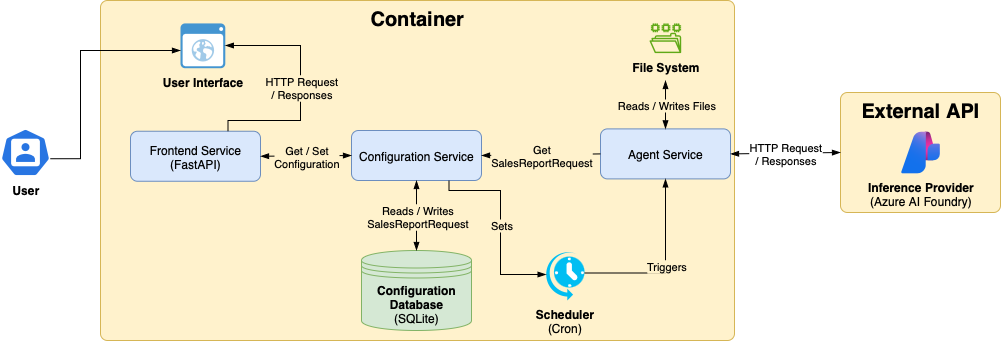
\includegraphics[width=1\textwidth]{images/system-diagram.png}
\caption{System Design Diagram}
\label{fig:system-diagram}
\end{figure}

Following the principle of modularity, the system is composed of three main services, as can be seen in \autoref{fig:system-diagram}. Each of these services has a well-defined scope and thus can be modified with limited effect to the others.

At the core of the system is the Configuration Service. This service is responsible for managing the user's configuration for the AI Analyst --- how often it runs, which sets the Cron scheduler, and the scope of the reports it generates, called SalesReportRequest within the system, which are stored in a local SQLite Database. This Configuration Service is consumed by both the Frontend and Agent services.

The Frontend Service is responsible for the user interface, which is served to the user through a FastAPI application. This user interface has a single functionality, allowing the user to configure for their AI Analyst, as can be seen in \autoref{annex:user-manual}. 

The Agent Service is where the AI Analyst is defined. This service uses the Configuration Service to retrieve the SalesReportRequests it must execute, and while executing, makes extensive use of the File System to store and retrieve data. Additionally, as inference is provided by Azure, the Agent Service communicates with Azure AI Foundry through HTTP.

Finally, the system has been designed to run in a single container, implemented in Docker. As the AI Analyst needs access to a company's private data, it should be easy to deploy inside each company's private cloud.

\section{Implementation}
\label{sec:implementation}

The process of implementing the system was divided into two parts, both of which will be explored in detail in this section.

First and most importantly, the implementation of the AI Analyst as an Agentic system. As an exploratory proof-of-concept, this was implemented through an iterative process, defined by a series of experiments with agent architecture, prompts and context which form the backbone of the reflections in \autoref{chapter:reflections}. These experiments were grouped in two stages, which are described in detail in \autoref{subsec:ai-analyst-implementation}.

Separately, the implementation of the Configuration Service, as well as the user interface to update the configuration, which was a one-off implementation, described in \autoref{subsec:config-implementation}.

\subsection{AI Analyst Agent}
\label{subsec:ai-analyst-implementation}

Before detailing the process of building the AI Analyst, it is important to note a few practical challenges that influenced some key decisions, mostly related to A\&M's restrictions regarding sharing resources for developing the system, as mentioned in \autoref{chapter:requirements-analysis}.

First, the system needed to be developed using Azure's student subscription, which provides a total of USD100 in credits to be used across their platform. This subscription also limits the LLMs that can be accessed with these credits. Some of the highest-performing models, such as OpenAI's o3, were thus not available.

Second, in the time that A\&M needed to review what data they could share for development, it was agreed to use \cite{wideworldimporters2025}, a public dataset created by Microsoft to simulate entries in a company's database. This would be closer to the production setup, which would likely need to retrieve its data from a database. Due to Microsoft's restrictions this dataset had to be hosted on Azure, and ran at the relatively high cost of USD1/day while it was being used.

The client was later able to provide anonymised sales data in the form of a CSV file. Thus, the database was turned off and the evaluations and integration tests that used it were removed from the repository, but the code for the agent that can extract data from it was kept in the repository for the client's future reference.

Finally, due to the high cost of hosting the database it was decided to use a lower cost LLM to develop the system. Reasoning models can be up to 10 times more expensive than their non-reasoning counterparts, which would have increased the risk of reaching the account's spending cap. Consequently, while the system was being structured it used OpenAI's gpt-4o-mini model, and after the entire system was developed the model was changed to OpenAI's o4-mini, a reasoning model, for the final prompt engineering experiments.

\subsubsection{Single Task Architecture}

Considering the advances in agentic architectures mentioned in \autoref{sec:research-llms}, the first group of experiments attempted to leverage \cite{fourney2024magenticone}'s Magentic-One orchestration architecture, without modifications, to create a single task for retrieving and analysing data. This architecture is depicted in \autoref{fig:magentic-one-architecture}, and was implemented using Microsoft's Semantic Kernel framework, which exposes its own implementation of the Magentic-One architecture.

\begin{figure}[h]
\centering
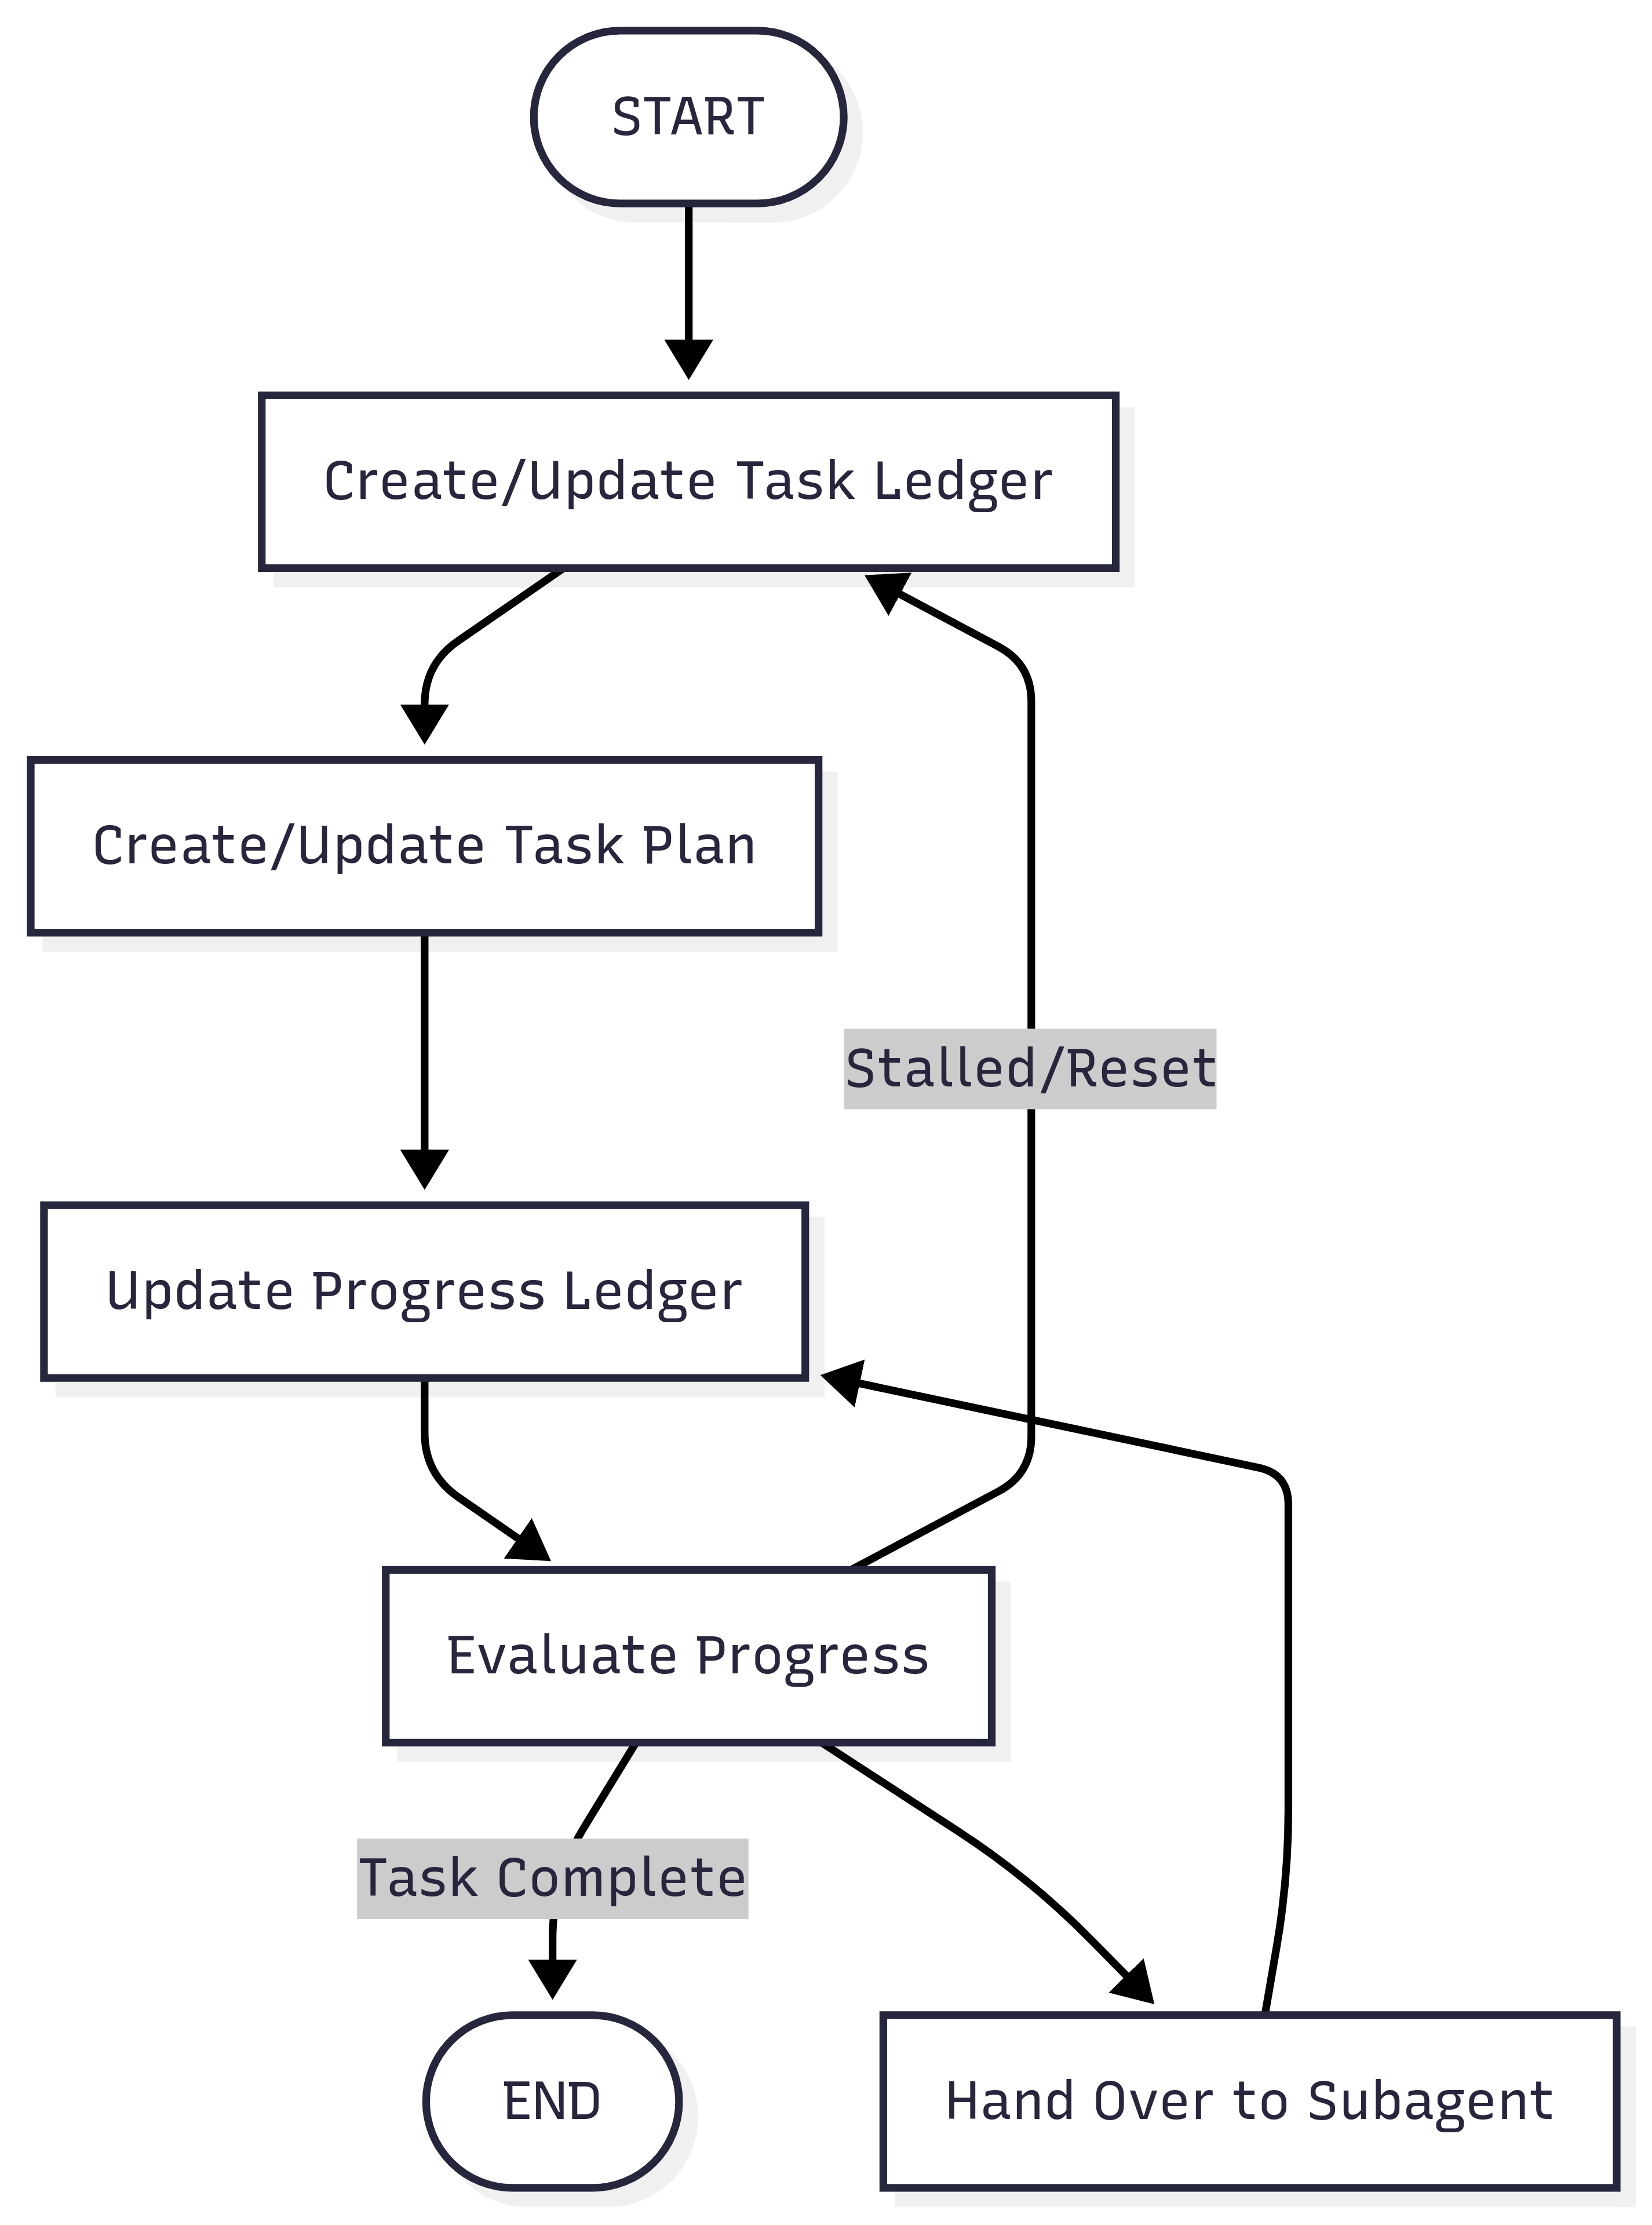
\includegraphics[width=0.4\textwidth]{images/mangentic-one-simplified.png}
\caption{Magentic-One Orchestration Architecture}
\label{fig:magentic-one-architecture}
\end{figure}

The key motivator for this approach was extensibility. With this orchestration architecture, adding new sources of information to the analysis would only require creating a subagent that can retrieve it and adding it to the team of subagents; the rest of the architecture could remain as it was. To start this team, three initial subagents were defined:

\begin{enumerate}
    \item A \textbf{Database Agent}, which had access to a tool to explore the tables in a database and execute arbitrary SQL queries. This agent used SemanticKernel's ChatCompletionAgent, their default way to create agents with any LLM as a reasoning engine.
    \item A \textbf{Coder (or Quantitative) Agent}, which had access to a code interpreter tool and thus could run arbitrary code. This agent used Azure's pre-defined agents, as this is the default way to access a code interpreter tool in the framework.
    \item An \textbf{Editor Agent}, with a system prompt detailing the structure and editing guidelines of the report. This agent also used SemanticKernel's default ChatCompletionAgent, without tools.
\end{enumerate}

The first challenge with this architecture, which became apparent as the first few attempts to run a full experiment were unsuccessful, was the integration of the Database Agent. The Database Agent in this instance is essentially a text-to-sql tool, and thus needed requests to be defined as queries for information. Magentic-One, however, defines the requests to the next subagent as tasks --- to give an idea, the request might be something like ``Investigate the main contributors to sales", but the Database Agent worked best with a query such as ``Retrieve sales by product family". Moreover, the default implementation of Magentic-One passes the entire conversation history as context to every subagent, but the Database Agent worked best with a minimal context.

The solution to this was to create another agent, an \textbf{Internal Data Agent}, which could access the Database Agent as a tool. In this architecture, the Internal Data Agent could receive a task, including the entire conversation, break the task down into a set of natural language queries, and request them one by one to the Database Agent. The advantage of using the agent-as-tool architecture was that the Internal Data Agent did not need to know how its text queries were executed, increasing the modularity of the design; the Database Agent could be changed for any tool that retrieves data based on a plain text query.

Another interesting question was where to use the Editor Agent, that is, whether to include it in the team of subagents for the Magentic-One task, or as a separate step that would take the results from the research task and generate the formatted report from it (similar to a traditional RAG architecture). After experimenting with both, including the Editor Agent within the Magentic-One task resulted in reports that missed more of the editing guidelines. Again, it seemed like the culprit was the increased context included in each request, in line with \cite{veseli2025positionalbiasesshiftinputs}'s findings.

This then set the architecture for the Single Task approach as a two-step flow. First, a Magentic-One task for retrieving and analysing all the information required, using a team of two agents: the Internal Data Agent, which in turn used the Database Agent as a tool, and the Quantitative Agent. Second, an editing step where the Editor Agent generated the formatted report using the results from the task as context.

After setting the architecture, the agent's output could be improved through prompt engineering. While the experiments with prompts were limited in this stage, as it was quickly clear that the system would need a different architecture, this process left an interesting question for the next stage: should prompts be tailored specifically to the sales task, or should they be general enough that they could be reused for any KPI?

Some of the first prompt attempts followed the second philosophy, attempting to be written in a way such that changing only one phrase could make them a viable task description for any KPI. This meant using ``zero-shot'' prompts, avoiding examples specific to sales. These prompts were generally not successful, though, which is in line with commentary on both the literature and prompting guides by LLM providers; the results were easily improved just by providing examples on the type of data that could be retrieved for a sales report, and this was the approach taken for the rest of the project.

It is possible to envision a prompt module that is designed so that it is easy to inject different examples or terms depending on the requested KPI; but as the proof-of-concept only needed to extract Sales information, this was not implemented.

\subsubsection{Workflow Architecture}

After a few experiments with the prompts for the Single Task Architecture, it was clear that some of the key nuances of the task were not being properly conveyed in the output. As such, the next stage of the project was to design a workflow that the agent could follow which reflected the ``standard operating procedure (SOP), with step-by-step instructions for how a human would perform the task or process'', as recommended by LangChain in \cite{langchain2025buildAgent}. Based on the author's experience in financial analysis, the workflow represented in \autoref{fig:workflow} was designed as the SOP for this task.

\begin{figure}[h]
\centering
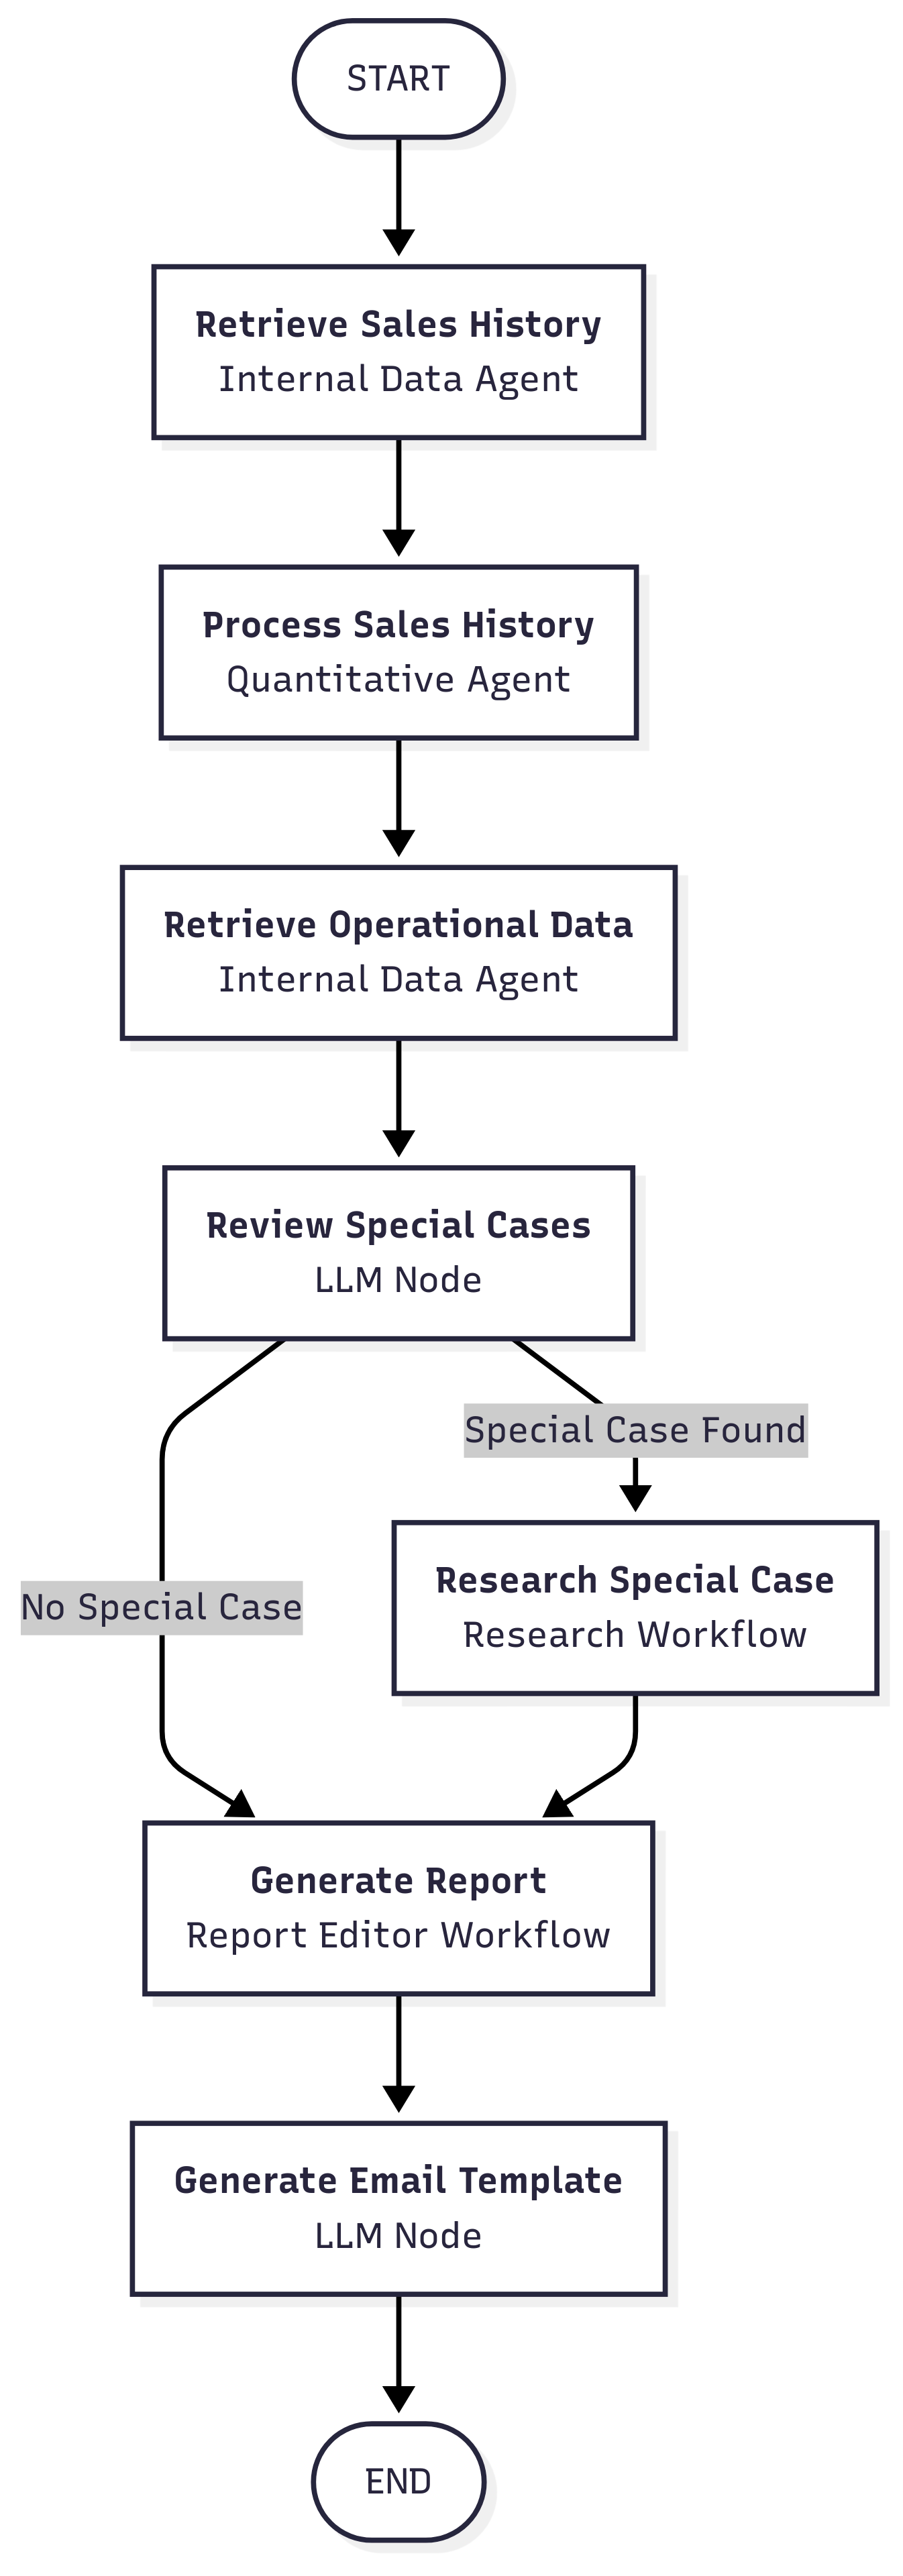
\includegraphics[width=0.3\textwidth]{images/workflow.png}
\caption{AI Analyst workflow, including agent or workflow that implements each step}
\label{fig:workflow}
\end{figure}

As the new workflow would not use Magentic-One as its core architecture, Semantic Kernel was not necessarily the best framework for structuring it. Changing frameworks had some downsides, however, as it would mean losing the functionalities already implemented, and the loss of Semantic Kernel's implementation of Magentic-One, which could be useful for some of the steps in the workflow. Working with Semantic Kernel, however, had already proven complex. It was not particularly intuitive for fine-grained control of agent's context, which was the main motivator of the architecture change, and it lacked community resources or documentation to support development for use cases that did not fall within its pre-defined structures. LangGraph, in contrast, is specifically designed for this kind of workflow oriented agentic workflow, and due to its popularity there is extensive community content. As such, it was decided to use LangGraph from this point forward.

It was also close to this point that the client was able to provide anonymised sales data for testing. As mentioned before, this was provided as a CSV file, so the Database Agent's function to the system could be replaced by an agent that could write and execute code in the environment that contained the CSV file.\footnote{Though as mentioned before the code for the Database Agent was kept in the repository for the client's reference.} Furthermore, allowing agents to read and write files from the file system could provide an easier way to pass down large tabular data between steps. Instead of storing all of them in context, which could easily exceed a model's token limits, intermediate outputs could be stored as CSV files within a temporary folder, and other agents would have access to them if needed. Thus it was decided that any agents that needed tabular data derived from this CSV would be created with tools that allow code execution directly in the container's environment.

Considering the change in both framework and data access, the new workflow was implemented iteratively, starting with a version that only included retrieving the sales history, processing it and creating a report. Further steps were then added to this base system one at a time. Each time a step was added or altered significantly, a full experiment and evaluation was performed, so that the impact of each change on the overall output was clear. This also confirmed the extensibility of the design, as additional steps could be added without breaking the existing functionality.

Following this iterative approach, the first versions of the workflow did not use custom architectures for its subagents. Instead, any agent that required tool usage, such as the \textbf{Internal Data Agent}, which now used a tool to run arbitrary code to retrieve data from the provided CSV file, and the new version of the \textbf{Quantitative Agent}, used LangGraph's implementation of the ReAct architecture. Additionally, while the Magentic-One architecture did not generate the expected results for the entire task, it was clear that it had value due to its extensibility and deep research capabilities, so it was used for the first implementation of the \textbf{Research Workflow} that executed the Research Special Case step --- that is, the step to explore the available data and find potential causes of special cases. These architectures would be customised based on the results of experiments, as described later in this section.

Also following this iterative approach, the first experiments used the Quantitative Agent to both analyse data and create visualisations in a single step. This resulted in visualisations that were poorly formatted despite variations on the prompts, so it was decided to separate plot generation from the analysis step. It then made sense to create a separate workflow for the generation of the report, the \textbf{Report Editor Workflow}, which consists of a Supervisor, which ensured task completion, a Report Writer, which contained the report's editing guidelines, a Data Loader, which can load a CSV file's contents into the workflow's context, and a Data Visualisation agent, which uses LangGraph's ReAct implementation and coding tool to generate and store plots.

After building this first version of the workflow, the LLM component was changed to the more expensive reasoning model, o4-mini. As was expected, reasoning models are better at complex tasks, and the change resulted in more detailed analysis. However, there was a drawback to the change: configurations that limit the range of potential results from the LLM, such as Temperature, Top P or Top K are not available for reasoning models. This resulted in an increased likelihood of agents getting stuck in infinite loops, even with the same prompts and data --- they would attempt to run code with errors without being able to fix it between loops, or request unavailable data time after time.

Some of these issues were improved upon with prompt engineering, such as providing clearer instructions on when to stop, but the stochastic component of LLMs meant there was no way of ensuring, just through prompts, that an infinite loop won't happen on any given experiment. As such, changes to the agent's architecture were needed.

\begin{figure}[h]
\centering
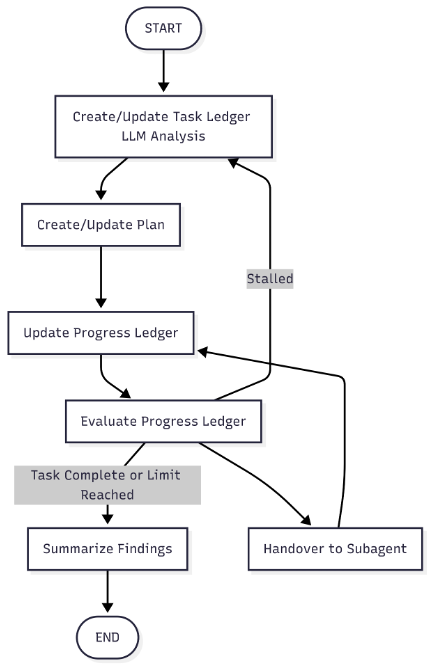
\includegraphics[width=0.4\textwidth]{images/research-workflow.png}
\caption{Research Workflow architecture.}
\label{fig:research-workflow}
\end{figure}

First, for the Research Workflow, which used the Magentic-One architecture, the main issue was that the model could not consistently decide that the task was complete. While a human would execute a judgment call considering that they have ``enough'' findings for the report, an LLM needs a clear stopping rule, which does not exist for a research task. Thus, it was decided to add a forceful exit condition, where the workflow would break the execution loop after a number of plan updates (note that this is different to progress ledger updates, which happen every time a sub-agent returns a response, plan updates only happen when the execution is deemed stalled by the orchestrator). This approach is in line with Semantic Kernel's own implementation.

Additionally, building from the learnings of the first stage of experiments, a Summarise Findings step was added to the Magentic-One workflow. Without this step, the best way to share the findings from the task would be to share the entire conversation, adding a large amount of context to the report generation step. Instead, by summarising the findings, only the actually relevant parts of this conversation, such as findings and files generated, are shared with the following step, maintaining the total size of the context contained. The final architecture for the Research Workflow can be seen in \autoref{fig:research-workflow}.

\begin{figure}[h]
\centering
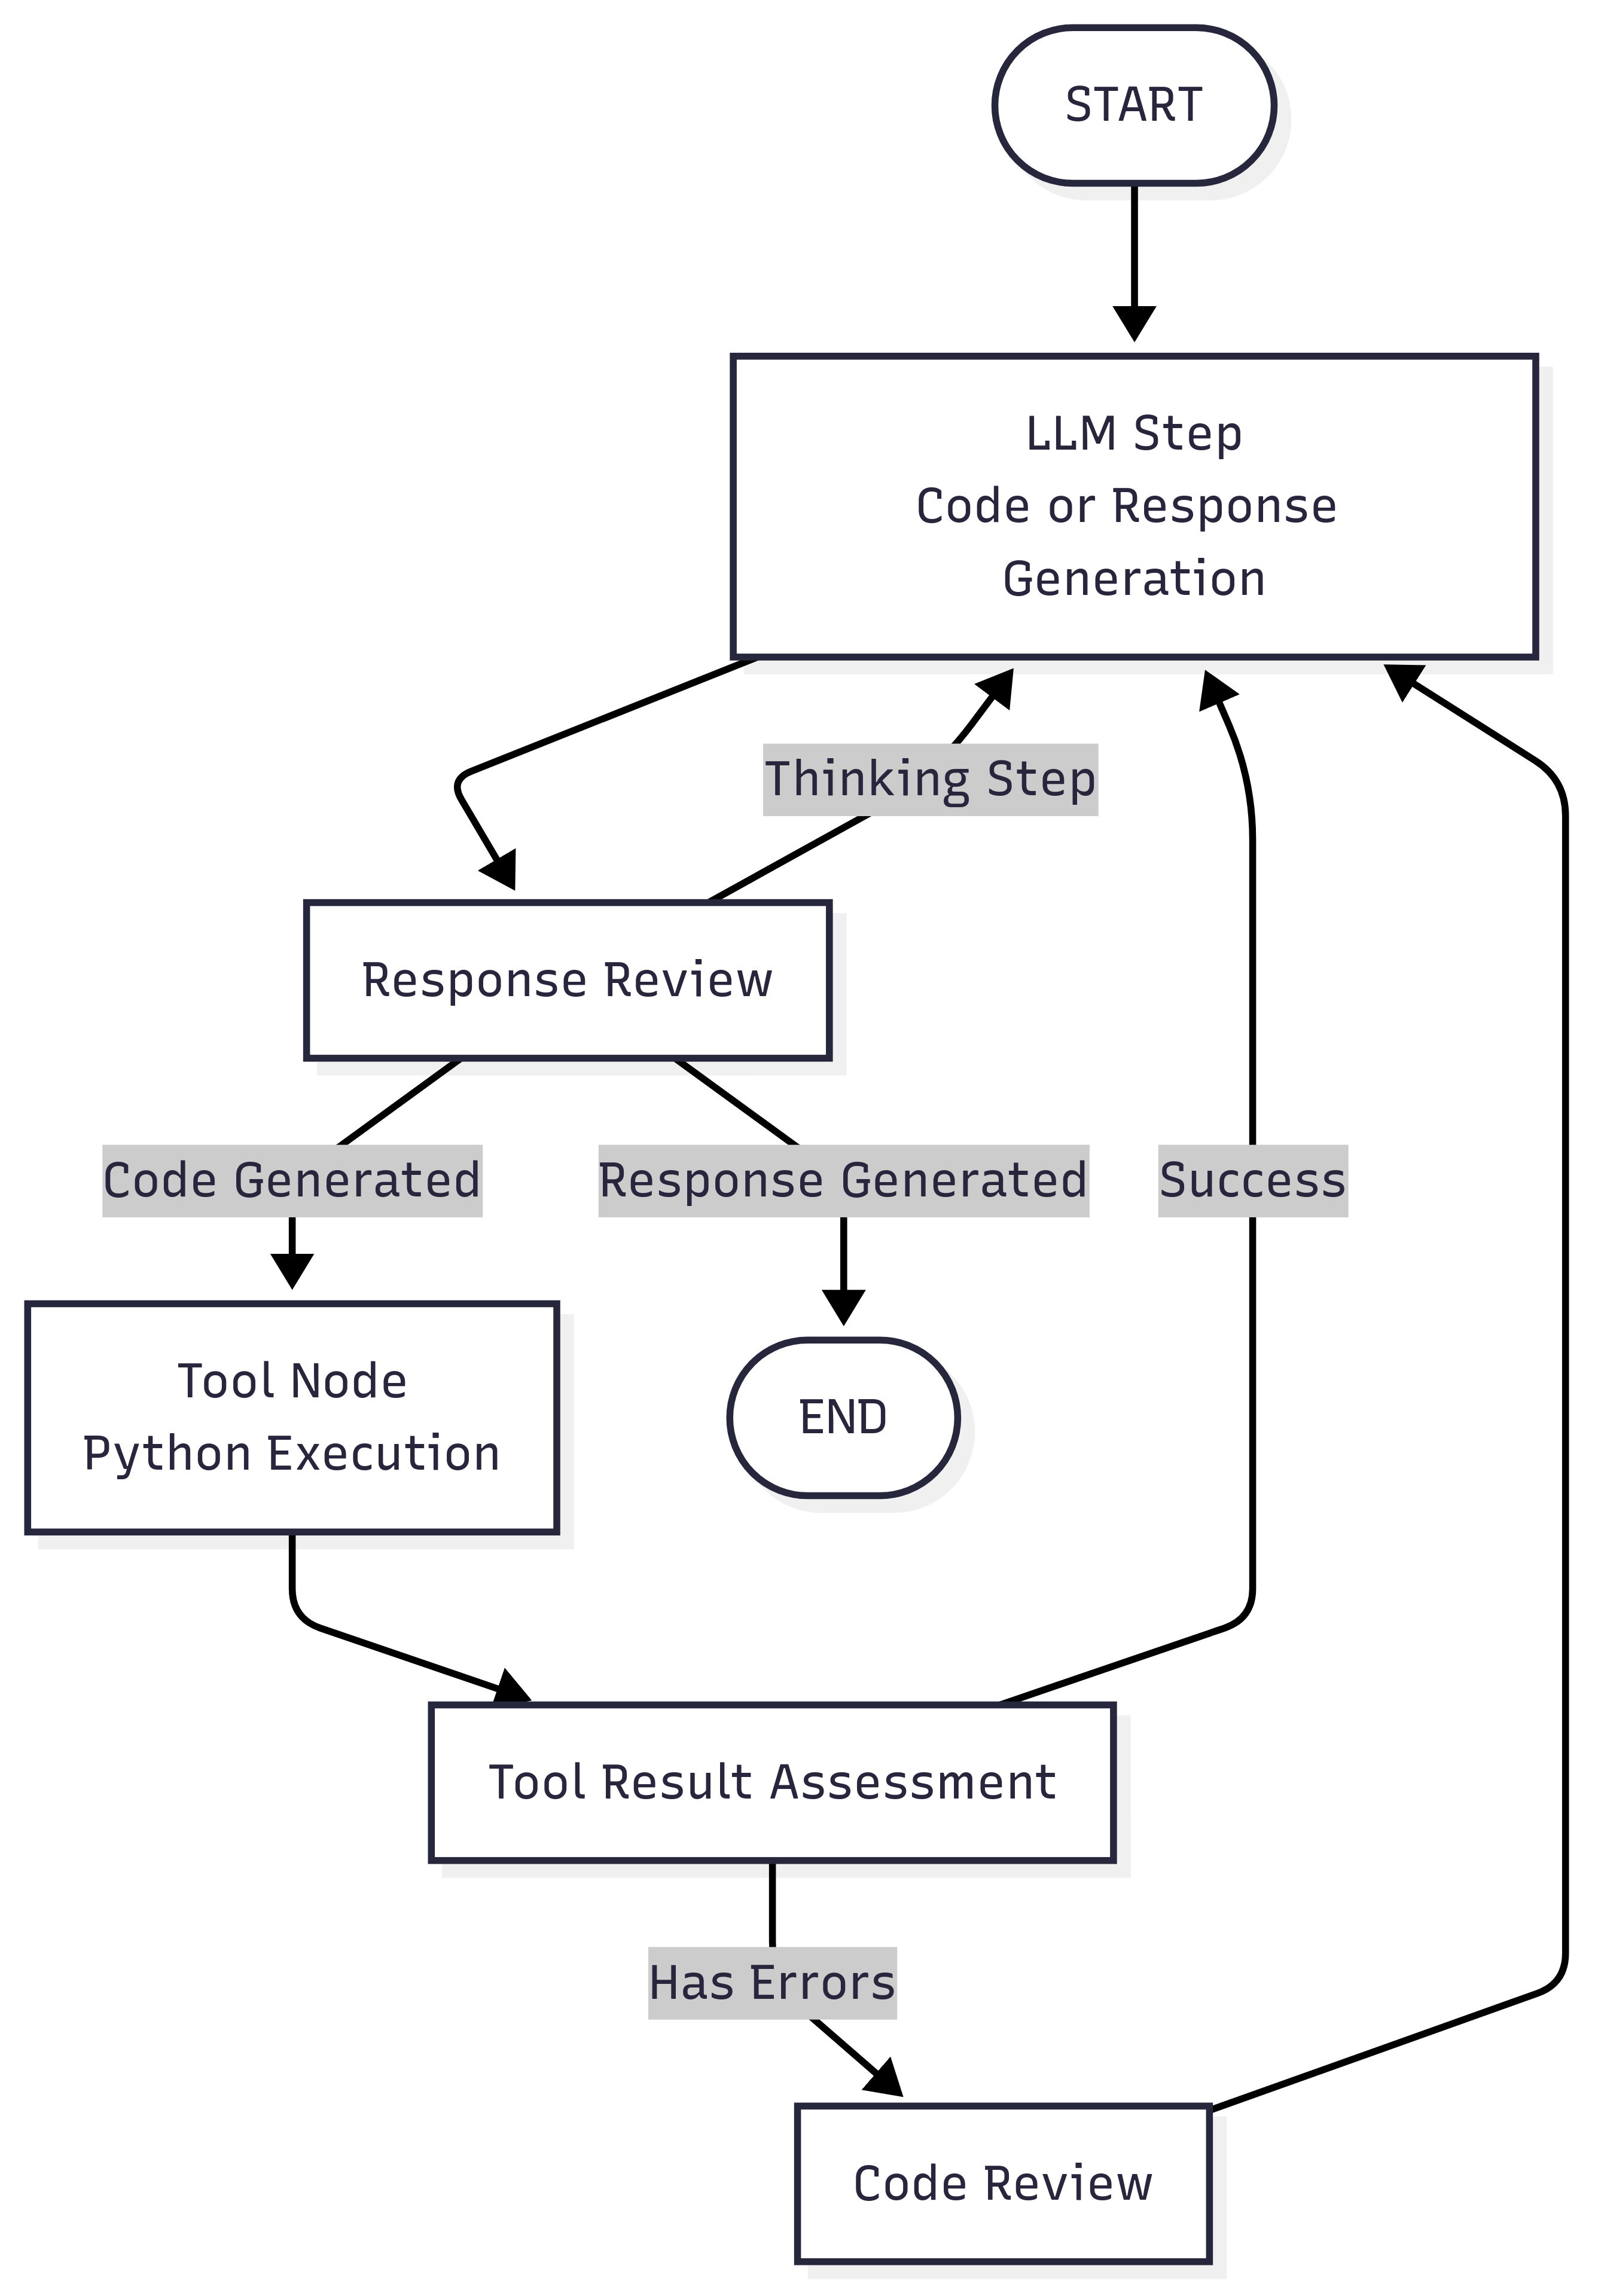
\includegraphics[width=0.4\textwidth]{images/coding-workflow.png}
\caption{Coding Agent architecture.}
\label{fig:coding-workflow}
\end{figure}

Second, both the Internal Data Agent and the Quantitative Agent generate code that needs to be executed in the local environment, using a Python Read-Evaluate-Print-Loop (REPL) Tool. For these agents, which first used a basic ReAct architecture, the issues were twofold. On one side, when the code generated had issues, such as error messages, the LLM would not consistently find the right fix, in some instances leading to hundreds of loops with the same error. On the other side, the LLM would sometimes return an intermediate thinking step without a tool call. In a default ReAct agent this is assumed to be a final response, and thus the task would remain incomplete.

To improve the agent's self-recovery capabilities, a new architecture, inspired by \cite{shinn2023reflexion} was defined. This architecture includes a step where the code outputs are reviewed for errors. If errors are present, a separate LLM is requested to provide a code review, which is added to the agent's context before looping. Additionally, when an error is detected a number of times in a row, or the agent has looped more than an allowed number of times, the prompt for the next loop is changed for one that requires the LLM to review its attempts, analyse what went wrong and provide this analysis as a final response. This approach is particularly useful when the agent is included in the Magentic-One orchestration, as it can provide information to the orchestrator for either retrying the request or changing its plan.

To avoid early returns due to thinking steps, the architecture includes a step that reviews the response from the agent. If the response includes a tool call for code execution, it moves to the tool execution step. If the response is only text, it is reviewed by an LLM to decide whether it is meant as a final response, in which case it is returned, or as an intermediate thinking step, in which case the loop starts again.

These additional steps have a key trade-off, they make the agent more expensive and slower to run, but reduce errors. Nevertheless, as the system is designed to run as a scheduled task, adding latency does not affect user experience. The extra cost could be reduced by using a non-reasoning model for these additional reviews, as neither is a complex task, so gpt-4o-mini was used.

The final architecture, which can be seen in \autoref{fig:coding-workflow}, was implemented as a reusable agent that can be initiated with any system prompt. This made it easy to use it for both an Internal Data or a Quantitative Agent, reducing potential duplications.

\subsection{Configuration Service and Interface}
\label{subsec:config-implementation}

The Configuration Service is, in practice, a module within the system, which is imported and used by the other services according to their needs. This module is responsible for three things:

First, it is responsible for loading the system's settings, such as API keys, from the environment or a \texttt{.env} file. As FastAPI uses Pydantic for type validation, it was an easy decision to use Pydantic's \texttt{pydantic\_settings} library to validate the presence and types of environment variables --- using this package ensures the system will fail on startup if the environment is set incorrectly. Similarly, this module is used to set up any system-wide constant, such as the location of data and temporary files.

Second, it is responsible for handling setting and updating the Cron job that runs the AI Analyst according to the user's preferences. The system uses the \texttt{python-crontab} library for this purpose.

Finally, the service is responsible for storing, retrieving and updating user preferences regarding the report to be generated. The preferences are represented in code as a Pydantic class called SalesReportRequest, which includes attributes for the characteristics of the scope of the request and for the list of emails that should receive the report when generated. The key decision to make for this functionality was how to persist these SalesReportRequests.

While it was clear that setting up an external database was unnecessary overhead for storing a local configuration, two alternatives were contemplated: serialising instances of the class and storing them as files, or storing them in a sqlite database within the same container.

Serialisation would have been the easiest option to set up, and should have performed well for the needs of the proof-of-concept, which only handles a few reports. Nevertheless, it was decided to use a local sqlite database as it would be more robust if the system is ever implemented within a large company, as A\&M's clients usually are. A large company may have hundreds of sales managers setting up their reports and, while databases can handle this without any issue, there is a high risk of file corruption if users make concurrent attempts at updating the configuration.

Considering this, a simple database was defined with two tables: \texttt{sales\_report\_requests} and \texttt{recipient\_emails}, sharing a one-to-many relation (one report request can have many recipients). Additionally, following the principle of extensibility, it was decided to use an ORM (\texttt{sqlalchemy}) for handling this database, as it would make the system easier to connect to a different database or add additional configuration if needed --- for example, some type of user authentication.

\subsubsection{User Interface}

To update the Configuration, a frontend was implemented as a FastAPI web application using Jinja2 templates. This implementation also follows a modular architecture --- templates can easily be changed to suit the preferences of any company that uses the AI Analyst, without affecting the rest of the system. The initial templates created consider the analysis in \autoref{chapter:requirements-analysis} and as such try to be simple and intuitive, using Bootstrap 5 to speed up implementation.

The FastAPI application consists of three main router modules as detailed in Table \ref{tab:frontend-routes}:

\begin{table}[H]
\centering
\begin{tabular}{|p{2.5cm}|p{5.5cm}|p{6.5cm}|}
\hline
\textbf{Router} & \textbf{Routes} & \textbf{Functionality} \\ \hline
\textbf{Index Router} & 
\texttt{GET /} \newline \texttt{POST /run\_now} & 
Main dashboard displaying existing Sales Report Requests and cron schedule configuration, as well as a form to update the cron schedule. Includes a route to run the agent immediately for testing. \\ \hline
\textbf{Sales Report Router} & 
\texttt{GET /sales\_report/create} \newline \texttt{POST /sales\_report/create} \newline \texttt{GET /sales\_report/edit/\{id\}} \newline \texttt{POST /sales\_report/edit/\{id\}} \newline \texttt{POST /sales\_report/delete/\{id\}} & 
Complete CRUD operations for Sales Report Requests, including a route that serves a form for creating or updating. \\ \hline

\textbf{Cronjob Router} & 
\texttt{POST /crontab/update} & 
Manages the cron schedule configuration for automated report generation. \\ \hline
\end{tabular}
\caption{Frontend Router Structure and Functionality}
\label{tab:frontend-routes}
\end{table}

\chapter{Evaluation and Testing}
\label{chapter:evaluation-testing}

As mentioned before, this project followed \cite{aiebook2025}'s recommendations regarding LLM evaluations. These included following Evaluation Driven Design, or the practice of writing the evaluations before working on the agent, as well as evaluating the components of the agent separately.

As such, \autoref{sec:agent-evals} will discuss the evaluation framework designed for the AI Analyst's output, which was defined before the start of implementation, and \autoref{sec:components-evals} details the approach taken to the evaluation of the agent's components. \autoref{sec:other-tests} discusses the approach taken to test for the non-agentic parts of the system, such as the configuration module.

\section{Agent Output Evaluation}
\label{sec:agent-evals}

Knowing the complexities of prompt and context engineering, developing a consistent way to evaluate the outputs of the AI Analyst was essential for the development process, as it would ensure that iterations could be performed safely, and improvements, or regressions, could be objectively defined. Yet, in line with the research described in \autoref{sec:research-llms}, evaluating the AI Analyst posed a series of challenges.

First, even for a single type of Sales Report Request, it would be impossible to create a comprehensive set of all possible valid reports that could be generated, so the traditional Machine Learning strategy of evaluating against ground truths was not viable.

Second, evaluating task completion was not relevant. With the current state of LLMs, obtaining a report is relatively straightforward; the greater challenge lies in ensuring that the report is actually what the users would expect, that is, it has the structure expected, the data extracted is correct and the insights are relevant. Moreover, it would be ideal to evaluate how useful the contents of the report are for decision making, but it would be extremely complex to define this beforehand --- different situations might require different data to make a decision, and in many cases only the actual decision maker would be able to provide feedback on whether the report was enough for them.

Considering these challenges, it was decided that the best path was using a ``subjective evaluation''. That is, having an external validator that would take the report generated, review it and grade it. This grading could consider the particularities of the task, and could act as a north star for development: higher scores could mean forward progress.

But, because the scope of the project is only a proof-of-concept, the evaluations defined are unlikely to be used in the final system. In fact, having an evaluation module was not even part of the client's requirements. It was thus important to limit the effort dedicated to creating the evaluation framework.

Due to this, it was decided to use a human judge as evaluator. While LLM judges have advantages, particularly the potential of running autonomously and thus increasing the number of iterations performed, setting up an AI Evaluator added unnecessary complexity at this stage, namely, the need to set up additional evaluations --- it would add the need to ``evaluate the evaluator'' to make sure that its grading is accurate.

Knowing that outputs would be evaluated by a human, the key challenge became ensuring that the score accurately reflected the needs of the task, specially considering the findings of \cite{hu2023decipher} regarding potential biases in human evaluation. The solution was to use a tried-and-tested framework from education: a grading rubric\footnote{Thanks to Professor Griffin for his comments that pointed in this direction.}. In essence, this grading rubric could contain the most relevant aspects of the report and assign a grade to each, thus producing an overall grade. 

\subsubsection{Rubric Definition}

When evaluating an LLM application, \cite{aiebook2025} recommends thinking of three groups: Domain-Specific Capacity, Generation Capacity and Instruction-Following Capacity.

In the context of a report, it is possible to think about Instruction-Following as the capacity of the agent to output a report that follows the structure and editing guidelines provided to it, and Generation as the capacity to retrieve and present the correct data. Both of these can be considered as part of the \textit{form} of the report --- does the report include the right sections, is the data correct and not hallucinated, is the data presented graphically, etc.

On the contrary, Domain-Specific Capacity in this context can be considered the capacity of the model to perform financial and operational analysis, such as accurately representing the evolution of an indicator instead of just mentioning its value, or only presenting relevant data. These are more reflective of the \textit{content} of the report.

This defined the two groups of questions to be included in the rubric: questions related to the \textit{form} of the report, and questions related to its \textit{content}. Moreover, in addition to the total score for the rubric, each group of questions is used to calculate its own score.

After defining this general structure of questions, the main challenge for the evaluation rubric was to define the level of specificity of its questions. If the questions included were too specific, the evaluation would only become valuable for specific scenarios, but very open-ended questions increase the risk of subjective grading.

This was solved by defining questions that are wide in scope, but allowing only a Yes or No answer, in the style of ``Does the analysis in the report accurately represent the evolution of the KPI?". While this question requires reviewing the entire report, and subjectively defining what ``accurate" is, there is less risk that the same evaluator can have different responses to similar outputs, unlike if required to provide a specific grade.

Moreover, this type of question had two added benefits. First, it made it easier, and thus quicker, to evaluate a specific report. Second, it simplified the score definition --- the total evaluation score could be calculated as the percentage of positive responses over the total number of questions.

Thus, the final rubric, which can be found in \autoref{annex:evaluation}, consists of a list of 23 Yes or No questions --- 14 questions focused on the \textit{form} of the report, as this covers two types of capacity analysis, and 9 questions focused on its \textit{content}.

\section{Components Evaluation}
\label{sec:components-evals}

In addition to evaluating the final output, evaluating an Agent's components can help spot issues earlier in its development, or surface the causes of unexpected behaviour, even if it has most of the same challenges described before.

However, unlike with the final output, just evaluating the intermediate steps' completion could add valuable information, specially for development, as it allows to confidently build the system modularly without the need to run full experiments on every change --- a relevant issue when considering that full experiments could take up to one hour to provide an output as the system became larger.

Moreover, in many cases there is one aspect to the intermediate step that can act as a proxy for its utility to the system, such as making sure that a file is generated or that the output has a certain structure.

For these reasons, it was decided to use ``exact evaluation'' for the Agent's components. What's more, using strict rules to evaluate the results, such as confirming completion or that a file was generated, makes the evaluations similar to a regular test, and can be expressed as such in \texttt{pytest}, meaning these types of evaluation can be run automatically. Given this, 37 evaluations were written as part of the system's testing suite; you can find an example in \autoref{annex:sample-eval}.

One of the biggest challenges of this approach is that while the evaluations are \textit{expressed} as tests, they are not actual tests and should be interpreted differently. In some cases, the evaluation rule might check that a specific word or numeric value is included in the test --- this is specially useful when evaluating summarisation steps --- but that expected text might not always be present, or be present in a different format, due to the probabilistic nature of LLMs. In such cases, a failing ``test" does not mean the system is not working; instead, it means that a more detailed experiment needs to be run for the specific component.

A solution to this issue is to use a subjective evaluation that can also run automatically, such as using an LLM as judge, but as mentioned before this has additional challenges which are out of scope of this project.

Another unexpected challenge of using this strategy was handling the file system for tests. As defined before, one of the most important implementation decisions was allowing agents to read and write files to store intermediate data, mostly in a temporary folder that is created for each request. The creation of this folder, as well as any request to know its path, was handled in a shared module.

Ideally, the testing environment should be isolated from the rest of the application, which meant that it needed its own temporary folder, something that sounds easy but becomes difficult with the way \texttt{pytest} manages patching imported modules. Because modules in python are resolved the first time they are imported on a process, patching a shared module requires special care --- things like never importing at the module level, and transitively patching when a module imports a module that imports the patched module. While this was solved for this version of the system, if development will continue it would be worth considering a simpler way to set up tests, as this can slow down development as the system becomes more complex.

Finally, the biggest issue with this approach is how long it takes to run the test suite. Evaluations expressed as tests are essentially integration tests; they perform real calls to the model provider, facing latency, and evaluated subagents perform real, if reduced, tasks, which might take several loops of the agent. This discourages running the entire evaluation suite on code changes, thus sometimes voiding the benefit of identifying unexpected regressions from a change. A production version of the system might benefit from splitting pure tests and evaluations as two suites that do not have to run together.

\section{Other Tests}
\label{sec:other-tests}

While the LLM components of the system need to be evaluated, an Agent is also composed of parts that are indeed subject to traditional tests; for example, some of the tools it uses are deterministic, and the integration with model providers is as well. Furthermore, the entire system goes beyond the AI Analyst Agent. Its other, more traditional software components also need testing.

Nevertheless, as mentioned a few times already, as a proof-of-concept, iteration speed outweighed testing completeness, as this system might face significant changes before becoming production-ready. As such, the approach taken to testing can be summarised as:

\begin{enumerate}
    \item Focus on unit testing, with some narrow integration tests.
    \item Avoid writing tests for functionalities that only wrap external libraries, such as email sending or PDF generation. It is assumed that the libraries themselves are well tested.
    \item For the most important functionalities, such as the configuration modules, 100\% coverage was ensured.
    \item For less critical functionalities, only testing the ``happy path'' was acceptable.
    \item For the frontend, as it is expected to completely change when integrated to a company's systems, manual acceptance testing was considered acceptable.
\end{enumerate}

Considering this, 23 tests were written for the configuration module, as it was considered the most critical part of the system, 17 tests were written for functionalities related to the agent execution, such as tools and utilities, and 5 unit tests for the frontend. The result of those tests, as well as the coverage summary, can be found in \autoref{annex:test-results}.

\chapter{Reflections}
\label{chapter:reflections}

The aim of this project was to explore the capabilities of AI Agents to act as a junior data analyst within a company. This was done by creating a proof-of-concept system, or AI Analyst, that can autonomously access a company's sales data, retrieve operational figures, extract initial insights from these figures and generate a sales report according to a user's sales scope.

There are thus two outputs from the project. The first is the proof-of-concept system, with the set of requirements discussed in \autoref{chapter:requirements-analysis} as well as its evaluation results. The other, perhaps more important, is the set of insights from building the proof-of-concept system, about using AI Agents for this type of task, which will be useful for the client's future projects.

\autoref{sec:requirements-achievement} will reflect on what was actually implemented in the system, compared to its requirements. \autoref{sec:key-insights} will reflect on the system's evaluation results and highlight the key learnings from the process. Finally, \autoref{sec:future-work} will reflect on how the proof-of-concept system can be improved to create a production-level application.

\section{Proof-of-concept Requirements Achievement}
\label{sec:requirements-achievement}

As can be seen in the following tables, the implemented system achieved 100\% of both Must Have and Should Have requirements, and one of the two Could Have requirements.

The Could Have requirement that was excluded from the proof-of-concept was FR-6, providing a sales forecast considering the remedial actions proposed by the agent. This requirement was not deemed possible with the current workflow definition, as the agent did not reliably provide measurable remedial actions for special situations. However, it should be possible to implement in a following iteration of the system, following the insights described in \autoref{sec:key-insights}.

Additionally, the system can generate reports on Total Sales --- a KPI relevant to a CFO-type user --- demonstrating its potential as a foundation for developing functionality for this type of user. However, implementing CFO-specific features was beyond the scope of the proof-of-concept.

% Define counters
\newcounter{ref-frcounter}
\newcounter{ref-nfrcounter}

% Formatting for IDs
\newcommand{\rfrid}{FR-\arabic{ref-frcounter}}
\newcommand{\rnfrid}{NFR-\arabic{ref-nfrcounter}}

\subsection{Functional Requirements}

\subsubsection{Sales Manager User}

\begin{table}[H]
    \centering
    \begin{tabular}{|l|p{8cm}|l|l|}
        \hline
        \textbf{ID} & \textbf{Requirement} & \textbf{Priority} & \textbf{Included} \\
        \hline
        \stepcounter{ref-frcounter}\rfrid & The system shall allow a Sales Manager-type user to set up a scope for their report & Must Have & Yes \\ \hline
        \stepcounter{ref-frcounter}\rfrid & The system shall be able to generate a Sales performance report based on the user’s preferences & Must Have & Yes \\ \hline
        \stepcounter{ref-frcounter}\rfrid & The system shall be able to identify “special cases” in Sales trends and perform a deeper analysis & Must Have & Yes \\ \hline
        \stepcounter{ref-frcounter}\rfrid & The system shall be able to provide simple Sales forecasts based on current trends & Should Have & Yes \\ \hline
        \stepcounter{ref-frcounter}\rfrid & The system shall be able to recommend potential actions to remedy “special cases” in Sales trends & Should Have & Yes \\ \hline
        \stepcounter{ref-frcounter}\rfrid & The system shall be able to provide simple Sales forecasts based on the remedy actions recommended by itself & Could Have & No \\ \hline
        \stepcounter{ref-frcounter}\rfrid & The system shall be able to provide advanced Sales forecasts using regression techniques or any other statistical method & Won’t Have & No \\
        \hline
    \end{tabular}
\caption{Sales Manager Type User Functional Requirements Achievement}
\end{table}

\subsubsection{CFO User}

\begin{table}[H]
    \centering
    \begin{tabular}{|l|p{8cm}|l|l|}
        \hline
        \textbf{ID} & \textbf{Requirement} & \textbf{Priority} & \textbf{Included} \\
        \hline
        \stepcounter{ref-frcounter}\rfrid & The system shall allow a CFO-type user to set up a list of KPIs they want their report to follow & Won’t Have & No \\ \hline
        \stepcounter{ref-frcounter}\rfrid & The system shall be able to generate a report for the user’s KPI list & Won’t Have & No \\ \hline
        \stepcounter{ref-frcounter}\rfrid & The system shall be able to provide simple forecasts for each KPI based on current trends & Won’t Have & No \\ \hline
        \stepcounter{ref-frcounter}\rfrid & The system shall be able to identify “special cases” in the trend of any KPI and perform a deeper analysis & Won’t Have & No \\ \hline
        \stepcounter{ref-frcounter}\rfrid & The system shall be able to recommend potential actions to remedy “special cases” in each KPI’s trend & Won’t Have & No \\ \hline
        \stepcounter{ref-frcounter}\rfrid & The system shall be able to provide simple forecasts for each KPI based on the remedy actions recommended by itself & Won’t Have & No \\ \hline
        \stepcounter{ref-frcounter}\rfrid & The system shall be able to provide advanced forecasts for each KPI using regression techniques or any other statistical method & Won’t Have & No \\
        \hline
    \end{tabular}
\caption{CFO Type User Functional Requirements Achievement}
\end{table}

\subsubsection{User Type Independent Requirements}

\begin{table}[H]
    \centering
    \begin{tabular}{|l|p{8cm}|l|l|}
        \hline
        \textbf{ID} & \textbf{Requirement} & \textbf{Priority} & \textbf{Included} \\
        \hline
        \stepcounter{ref-frcounter}\rfrid & The system shall email the resulting report to the email addresses configured by the user & Must Have & Yes \\ \hline
        \stepcounter{ref-frcounter}\rfrid & The system shall include both financial and operational information in a report & Must Have & Yes \\ \hline
        \stepcounter{ref-frcounter}\rfrid & The system shall be able to load information from a CSV file & Must Have & Yes \\ \hline
        \stepcounter{ref-frcounter}\rfrid & The system shall customise the email body with the key findings of the report & Should Have & Yes \\ \hline
        \stepcounter{ref-frcounter}\rfrid & The system shall be able to load information from other files provided by the user & Won't Have & No \\ \hline
        \stepcounter{ref-frcounter}\rfrid & The system shall be able to load information from a set of reliable online information sources & Won't Have & No \\ \hline
    \end{tabular}
\caption{User Type Independent Functional Requirements Achievement}
\end{table}

\subsection{Non-Functional Requirements}

\begin{table}[H]
    \centering
    \begin{tabular}{|l|p{8cm}|l|l|}
    \hline
    \textbf{ID} & \textbf{Requirement} & \textbf{Priority} & \textbf{Included} \\
    \hline
    \stepcounter{ref-nfrcounter}\rnfrid & The system shall be extensible to other sources of information & Must Have & Yes \\ \hline
    \stepcounter{ref-nfrcounter}\rnfrid & The system shall run autonomously at fixed intervals & Must Have & Yes \\ \hline
    \stepcounter{ref-nfrcounter}\rnfrid & The system shall allow the user to update the fixed interval at which it runs & Must Have & Yes \\ \hline
    \stepcounter{ref-nfrcounter}\rnfrid & The system shall provide a user interface to update its configuration & Should Have & Yes \\ \hline
    \stepcounter{ref-nfrcounter}\rnfrid & The system shall provide a user interface that is clear and easy to use & Should Have & Yes \\ \hline
    \stepcounter{ref-nfrcounter}\rnfrid & The system shall allow multiple users to set up their reports & Could Have & Yes \\ \hline
    \stepcounter{ref-nfrcounter}\rnfrid & The system shall allow users to authenticate before updating their report preferences & Won’t Have & No \\ \hline
\end{tabular}
\caption{Non-Functional Requirements Achievement}
\end{table}

\section{Evaluation Results and Key Insights}
\label{sec:key-insights}

% Counter for the key findings
\newcounter{kfcounter}
\newcommand{\kfid}{\textbf{Key Insight \arabic{kfcounter}}}

As mentioned in \autoref{chapter:evaluation-testing}, the AI Analyst's reports were evaluated using a rubric with 23 Yes or No questions about the contents of the report, which can be found \autoref{annex:evaluation}. The evaluation score for each experiment is the percentage of these questions that had a positive answer.

\autoref{fig:evals-total} charts the progression of the evaluation score, with separate curves showing the progression of the score for the \textit{form} and \textit{content} of the report, as well as the total score. The detailed rubric and results can be found in \autoref{annex:experiments}, and this section will explain the insights from these experiments.

\begin{figure}[H]
\centering
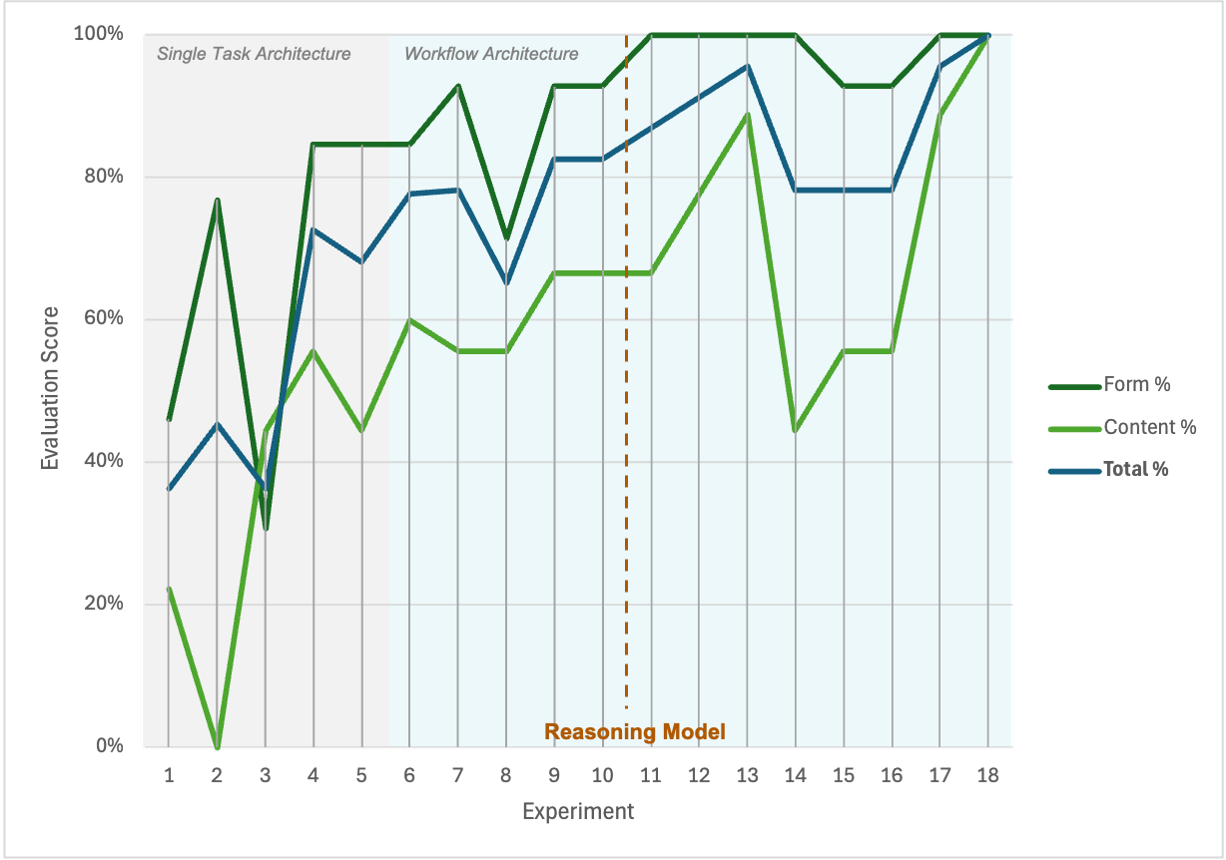
\includegraphics[width=0.8\textwidth]{images/evals-combined.png}
\caption{Evolution of evaluation results}
\label{fig:evals-total}
\end{figure}

As mentioned before, the first group of experiments attempted to use a single task architecture, applying Microsoft's Magentic-One orchestration with a task of retrieving and analysing all the information needed for the report. As evidenced in \autoref{fig:evals-total}, this approach could get a reasonably high score on the form evaluation, but never perfect. It consistently failed to properly present the ``current" period of data --- in every case, the report provided an analysis of the entire sales history, which is not useful for a report that will be issued periodically. This is a key nuance of the task.

Moreover, this approach failed to score more than 60\% on the content score, despite experiments changing both prompts and architecture. In fact, as can be reviewed in \autoref{fig:evals-detailed}, every iteration had issues with different parts of the content, making it hard to make targeted changes to improve results.

After an in-depth review of the intermediate steps taken by the system, the reason for this issue became clear: while the agent loops, all of its intermediate responses are added to its context, that is, the information sent with each request. This means that the agent's receives more and more information as it loops, even if the steps taken in each loop do not actually move the task forward. In this particular architecture, when the task is handed over to a subagent it includes the entire conversation history, so they received an enlarged context as well, making their responses worse as more loops take place. This led to two insights, which drove the approach to the second iteration:

\begin{itemize}
    \item \stepcounter{kfcounter}\kfid : LLMs can indeed perform large tasks with some success, but their effectiveness and reliability can improve by breaking the task into smaller subtasks.
    \item \stepcounter{kfcounter}\kfid : Deep research tasks increase the agent's context quickly, and the irrelevant context has a masking effect, so they benefit from summarisation steps within the workflow\footnote{As opposed to most common architectures which only summarise at the end of the task}. This is in line with the findings of \cite{veseli2025positionalbiasesshiftinputs}.
\end{itemize}

The first point can be seen clearly in \autoref{fig:evals-total}. After the change to a workflow architecture, fluctuations in form score reduced vastly, while the content score slowly increased as the entire workflow was rebuilt. This learning was solidified by the fact that the agent did not reliably provide measurable remedial actions. The request for remedial actions was included in the Research Special Case task, and the nuance for providing measurable actions was consistently lost within the growing context of this research workflow.

After finishing rebuilding the workflow, the system's default model was changed to use o4-mini, one of OpenAI's reasoning models, leading to \stepcounter{kfcounter}\kfid : changing to a reasoning model has a smaller impact on task completion than the change to a step-by-step workflow, as reasoning can be approximated through additional steps in the agent's architecture. It should be noted, however, that the quality of certain parts of the output, such as the visualisations generated, did improve markedly by using a more powerful model.

Additionally, as mentioned in \autoref{chapter:design-implementation}, with the change to a reasoning model the results became more volatile, as this type of model does not accept configuration variables such as Temperature, Top K or Top P. This was especially evident in the tendency of sub-agents to become trapped in infinite loops. This led to \stepcounter{kfcounter}\kfid : autonomous agents are not guaranteed to self-recover, and the system must be planned around that. Common architectures use steps to reflect and re-plan, but this assumes that the LLM will at some point deem the task complete. For cases such as deep research, where there might not be a clear measure for the task to be considered complete, it is important to create, and properly handle, forceful ending points.

Finally, as shortly discussed in \autoref{chapter:evaluation-testing} the evaluation score does not measure how useful the report is for decisions making, as it would be extremely complex to create a good measure for this. Some reports, for the same request and with access to the same data, might show detailed operational information by City and Product Family, while others might extract insights by Customer. All of these would get the same evaluation score, but might be more or less useful for the actual decision maker. This highlights \stepcounter{kfcounter}\kfid : with the current state of LLMs, they can be used to reduce the time spent in data extraction, but companies will still need a human in the loop to review the output, determine whether additional information is needed, and decide how to act based on the extracted insights.

\section{Future Work}
\label{sec:future-work}

The output of this project is an exploratory proof-of-concept system, it has access to anonymised data and is not deployed. As such, it can, and should, be improved upon before using in a production environment within a company. The most important changes to make this system production ready would be:

\begin{enumerate}
    \item Improvements to the evaluation framework:
    \begin{itemize}
        \item Fully automate the evaluation of outputs, to allow for quicker iterations.
        \item Evaluate intermediate steps within a full execution, in addition to individually.
        \item Add objective evaluation to intermediate steps when appropriate.
    \end{itemize}
    \item Improvements to the product readiness of the user interface for configuration:
    \begin{itemize}
        \item If the system will be deployed in a publicly accessible location, add authentication.
        \item Add acceptance tests that can be run on a CI/CD pipeline.
    \end{itemize}
    \item Improvements to the agent architecture and outputs:
    \begin{itemize}
        \item Make the corrective actions proposed by the LLM when there is a ``special case" measurable, by creating a separate step in the workflow dedicated to providing and measuring the recommendations.
        \item Research and implement ways for final users to provide feedback on the generated reports, particularly their usefulness for decision making.
    \end{itemize}
\end{enumerate}

\appendix

\printbibliography


\chapter{System Manual}
\label{chapter:system-manual}

This section provides the technical details necessary for developers to understand, deploy, and maintain the AI Analyst system. The system is implemented as a containerised Python application with clear separation of concerns across its core components.

\section{System Requirements}

The AI Analyst system requires the following technical environment:

\begin{itemize}
    \item Python 3.13 or higher
    \item uv package manager for dependency management
    \item Docker and Docker Compose for containerised deployment
    \item Azure account for AI model access (Azure OpenAI or Azure Foundry)
    \item SMTP server for automated email delivery
\end{itemize}

\section{Code Repository Structure}

The system follows a modular architecture with clear separation between agent logic, configuration management, and user interface components:

\begin{quote}
\texttt{src/}\\
\texttt{-agents/~~~~~~~~~~~\# AI agent implementations and workflows}\\
\texttt{-configuration/~~~~\# System settings and agent configuration}\\
\texttt{-frontend/~~~~~~~~~\# Web interface and API routes}\\
\\
\texttt{agent\_main.py~~~~~~\# Primary agent execution entry point}\\
\texttt{frontend\_main.py~~~\# FastAPI web application}\\
\texttt{data/~~~~~~~~~~~~~~\# Financial datasets}\\
\texttt{outputs/~~~~~~~~~~~\# Generated reports and artefacts}\\
\texttt{documentation/~~~~~\# Technical and user documentation}\\
\texttt{tests/~~~~~~~~~~~~~\# Test suite and evaluation framework}
\end{quote}

The source code is available at the project repository, with comprehensive documentation in the \texttt{documentation/} folder covering setup, architecture, and deployment procedures.

\section{Installation and Configuration}

System deployment follows a straightforward process:

Configuration is managed through environment variables defined in a \texttt{.env} file. Essential settings include AI model authentication keys, database connection strings, and email service configuration; see \texttt{.env.example}. The system uses Pydantic Settings for type validation, ensuring startup failures if the environment is incorrectly configured.

Dependencies are defined in \texttt{pyproject.toml}, and can be installed with a single command: \texttt{uv sync}.

Finally, the system includes a Docker configuration and thus can run as
\texttt{docker-compose up}.

\section{Data and Testing}

Test execution uses: \texttt{uv run pytest}. Note that the sample data is not included in the repository as it is too large, and thus the test suite will fail. Moreover, consider that the testing framework combines unit tests and agent evaluation, so it needs Azure API Keys to be set in the \texttt{.env} file before running.

\chapter{User Manual}
\label{annex:user-manual}

This manual provides a guide on how to use the Sales Report Setup user interface to configure your AI Analyst. It is organised by functionality.

\section{Getting Started}

Before setting up your AI Analyst, it is advised that you familiarise yourself with the user interface, which will look like \autoref{fig:frontend-empty} if you have not set up your Analyst yet, and like \autoref{fig:frontend-filled} if you have.

The upper section of the page allows you to run the AI Agent immediately with the ``Run Now'' button, and to add additional reports to be generated by the AI Analyst through the ``Create New Request'' button. See \autoref{annex:user-manual-report-request} for more detail.

\begin{figure}[H]
\centering
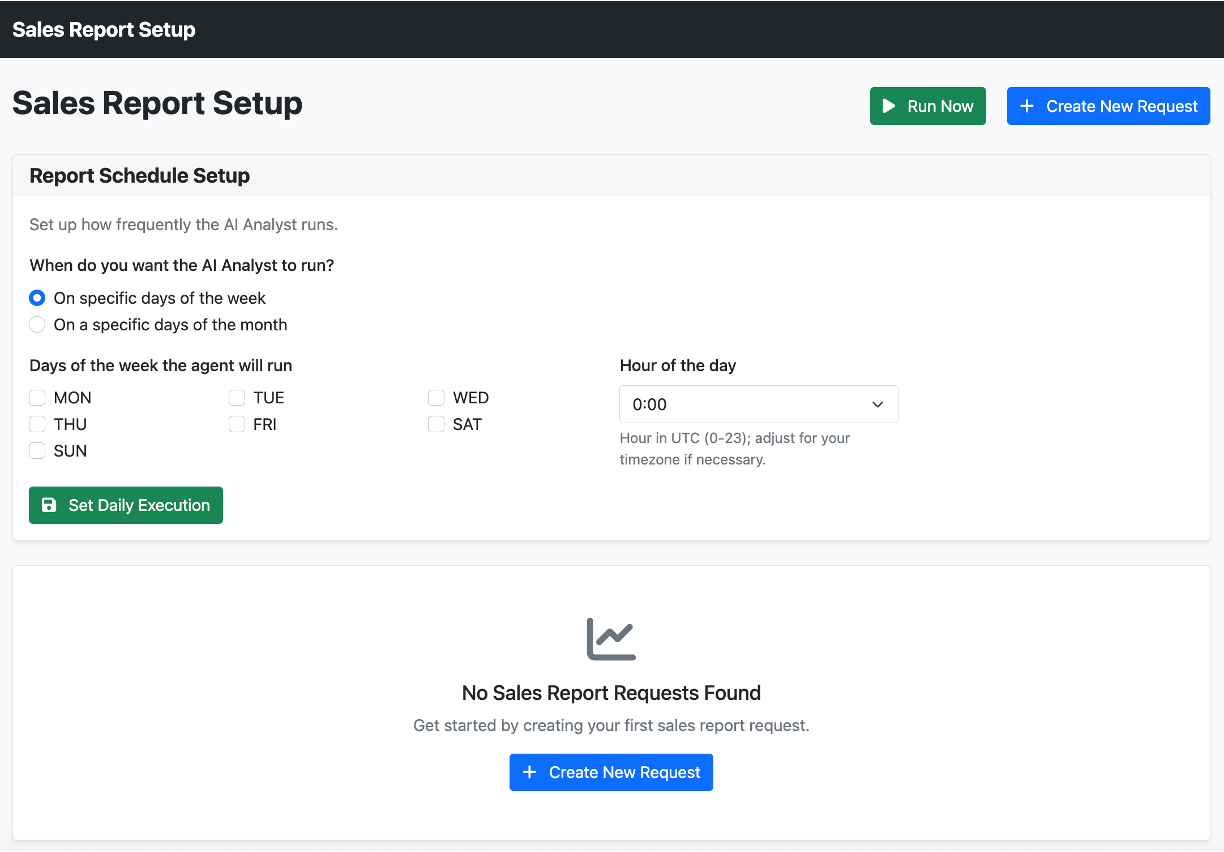
\includegraphics[width=0.8\textwidth]{images/frontend-empty.png}
\caption{User interface before any set up.}
\label{fig:frontend-empty}
\end{figure}

\begin{figure}[h]
\centering
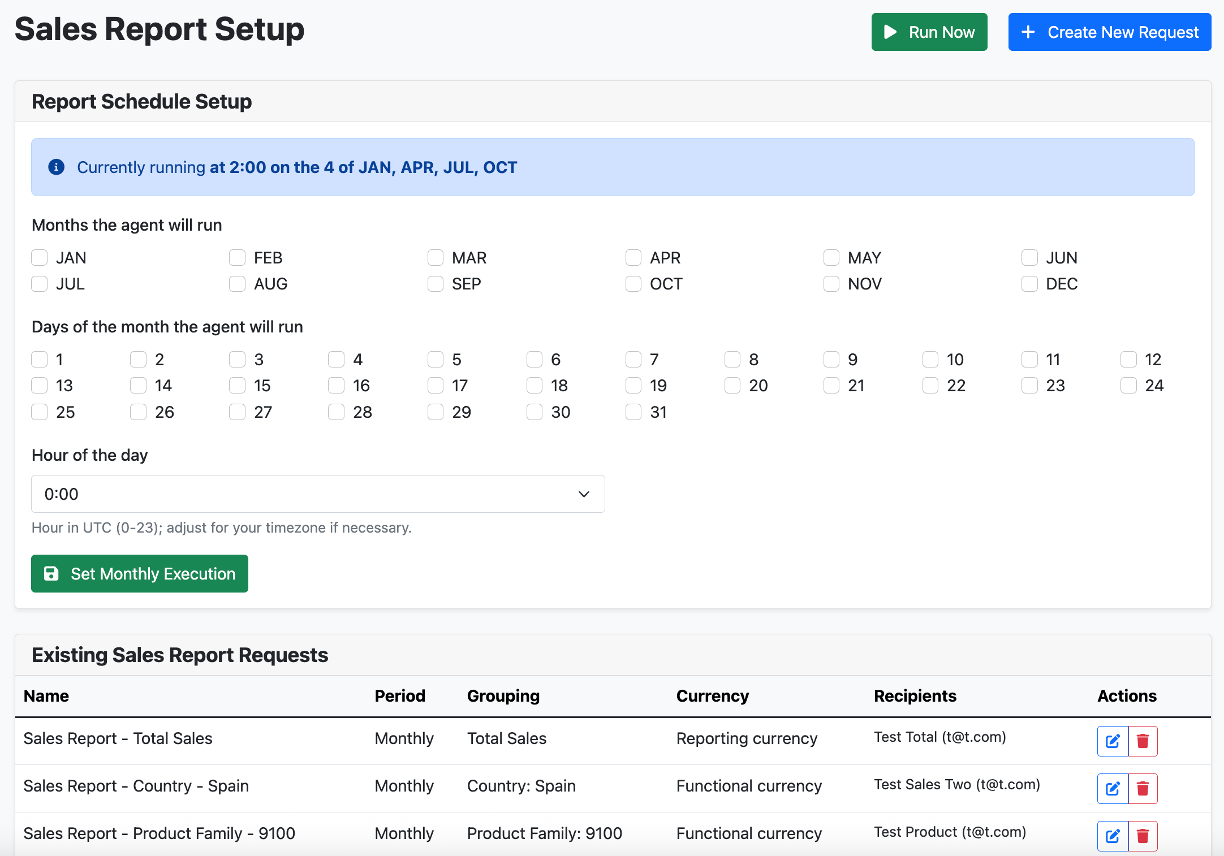
\includegraphics[width=0.8\textwidth]{images/frontend-filled.png}
\caption{User interface after set up.}
\label{fig:frontend-filled}
\end{figure}

\section{Scheduling Report Generation}

The top section of your screen is used for scheduling when the AI Agent will run, and thus generate your reports. You can select specific months and days. For example, you can select the months of January, April, July and October to receive reports quarterly.

After you have set up a schedule for your report, the current settings will be displayed, as you can see in \autoref{fig:frontend-filled}.

\section{Adding or Updating Report Requests}
\label{annex:user-manual-report-request}

When you click ``Create New Request'', you will be redirected to a screen that looks like \autoref{fig:frontend-form}. This is the form you will fill up to add a new report that you want to receive, or to update an existing one. The fields to set are:

\begin{itemize}
    \item \textbf{Period}: Whether the report covers Monthly, Quarterly or Yearly data.
    \item \textbf{Currency}: Whether the report should consider the Functional or Reporting Currency. This is only relevant for regions that use a different currency than the company's reporting currency.
    \item \textbf{Grouping}: Whether the report should consider sales by a specific product or geography. If not, select Total Sales.
    \item \textbf{Grouping Value}: If your report should consider only sales for a specific grouping, this is where you say which --- for example, the specific city or product.
    \item \textbf{Recipients}: The emails and names of the users that should receive the report.
\end{itemize}

When you finish filling the form, click ``Create Request''.

\begin{figure}[h]
\centering
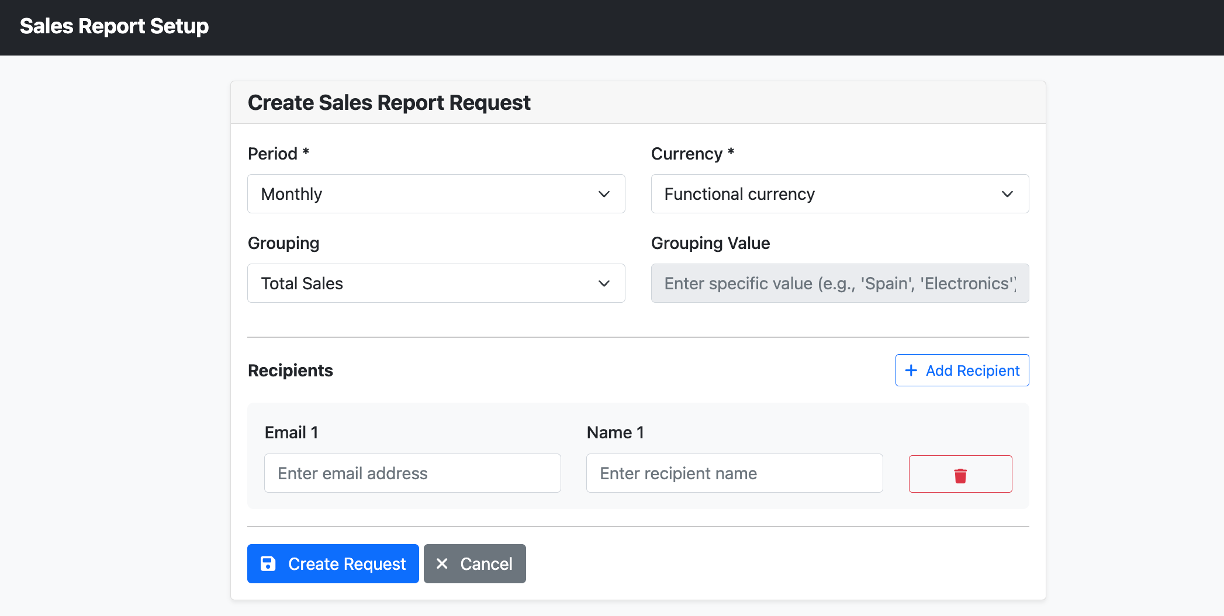
\includegraphics[width=0.8\textwidth]{images/frontend-form.png}
\caption{Sales Report Request setup form.}
\label{fig:frontend-form}
\end{figure}

If you have already set up one or more reports to receive, you will be able to see them in the main screen, as \autoref{fig:frontend-filled} shows. The buttons under ``Actions'' allow you to manage these requests. The left, blue button allows you to edit the report, while the right, red button allows you to delete reports you don't need any more. Note that when you edit the report, you will be redirected to a screen that looks like \autoref{fig:frontend-form}, but pre-filled with its current settings.

\chapter{Report Evaluation Rubric}
\label{annex:evaluation}

\begin{table}[H]
\centering
\begin{tabular}{|p{14cm}|}
    \hline
    \textbf{Form Items} \\ \hline
    Does the report include all the required sections? \\ \hline
    Does the report actually address the required KPI? \\ \hline
    Does the report include an analysis of the evolution of the KPI? \\ \hline
    Does the report include detailed data, in addition to the high level KPI information? \\ \hline
    Does the report include at least one graph? \\ \hline
    Does the report include more than one graph? \\ \hline
    Does the report include a projection of the KPI? \\ \hline
    Is the data retrieved correct? \\ \hline
    Does the report accurately present the last information period? \\ \hline
    Is the content of the Executive Summary accurate to the section's description? \\ \hline
    Is the content of the Overview accurate to the section's description? \\ \hline
    Is the content of the Trends \& Context accurate to the section's description? \\ \hline
    Is the content of the In Depth Analysis accurate to the section's description? \\ \hline
    Is the content of the Forward Outlook accurate to the section's description? \\ \hline
\end{tabular}
\caption{Checklist of \textit{form} Items}
\end{table}


\begin{table}[H]
\centering
\begin{tabular}{|p{14cm}|}
    \hline
    \textbf{Content Items} \\ \hline
    Does the analysis in the report accurately represent the evolution of the KPI? \\ \hline
    Does the report include an analysis of the detailed data? \\ \hline
    Does the detailed analysis mention specific drivers of decline? \\ \hline
    Are all graphs (visualisations) relevant to the report? \\ \hline
    Are all graph types adequate for the data presented? \\ \hline
    Are all projections adequate for the data presented? \\ \hline
    Does the report accurately note any ``special case'' present? \\ \hline
    Does the report provide next steps for any ``special case'' present? \\ \hline
Are all statements in the report sustained with data? \\ \hline
\end{tabular}
\caption{Checklist of \textit{content} Items}
\end{table}

\chapter{Experiments Performed and Evaluation Results}
\label{annex:experiments}

\begin{table}[H]
\centering
\begin{tabular}{|c|c|p{7cm}|c|c|c|c|}
    \hline
    No. & Date & Notes & Default Model & Form & Content & Total \\ \hline
    1 & 02-Jul & First test with all of my MVP Agents: Magentic-One (DB, Coder) + Separate Editor & gpt-4o-mini & 50\% & 29\% & 36\% \\ \hline
    2 & 02-Jul & Re-run of previous experiment & gpt-4o-mini & 75\% & 29\% & 45\% \\ \hline
    3 & 03-Jul & Move Editor Agent inside team, improve quant agent prompt & gpt-4o-mini & 50\% & 29\% & 36\% \\ \hline
    4 & 04-Jul & Improve Magentic-One task description & gpt-4o-mini & 75\% & 71\% & 73\% \\ \hline
    5 & 04-Jul & Improve Editor Prompt & gpt-4o-mini & 75\% & 64\% & 68\% \\ \hline
    6 & 09-Jul & First test with LangGraph --- Minimal MVP, without in-depth analysis & gpt-4o-mini & 78\% & 78\% & 78\% \\ \hline
    7 & 11-Jul & Add step for operational info just with the quant agent & gpt-4o-mini & 100\% & 64\% & 78\% \\ \hline
    8 & 15-Jul & Leave plot generation for last step & gpt-4o-mini & 67\% & 64\% & 65\% \\ \hline
    9 & 15-Jul & Re-run of previous experiment & gpt-4o-mini & 89\% & 79\% & 83\% \\ \hline
    10 & 23-Jul & Add the agent for in-depth research & gpt-4o-mini & 89\% & 79\% & 83\% \\ \hline
    11 & 24-Jul & Add the agent for in-depth research & o4-mini & 100\% & 79\% & 87\% \\ \hline
    12 & 28-Jul & Change prompt: `concise' to `detailed' & o4-mini & 100\% & 86\% & 91\% \\ \hline
    13 & 28-Jul & Re-run of previous experiment & o4-mini & 100\% & 93\% & 96\% \\ \hline
    14 & 29-Jul & Add capacity for report writing graph to load csv files & o4-mini & 100\% & 64\% & 78\% \\ \hline
    15 & 29-Jul & Re-run of previous experiment & o4-mini & 89\% & 71\% & 78\% \\ \hline
    16 & 30-Jul & Add check for coding agent intermediate input vs final input & o4-mini & 89\% & 71\% & 78\% \\ \hline
    17 & 30-Jul & Update prompt in quant agent to reduce intermediate requests for user input & o4-mini & 100\% & 93\% & 96\% \\ \hline
    18 & 31-Jul & Update prompt in internal data agent to ensure all files are generated in the right folder & o4-mini & 100\% & 100\% & 100\% \\ \hline
    \end{tabular}
\caption{Experiments performed with Evaluation scores}
\end{table}

\begin{sidewaysfigure}
    \centering
    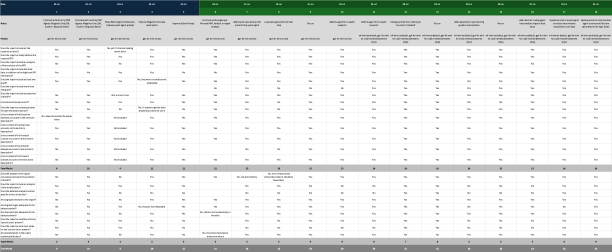
\includegraphics[width=\textheight]{images/evals-detail.png}
    \caption{Detailed evaluation scores; empty cells are items that do not apply to that specific experiment.}
    \label{fig:evals-detailed}
\end{sidewaysfigure}

\chapter{Sample Automated Evaluation}
\label{annex:sample-eval}

\begin{verbatim}
async def test_file_creation(quantitative_agent):
    """
    Test the agent creates at least one file in the temp directory.
    """

    query = f"""The company's sales for the last three years are as follows:' 
    
    {california_monthly_sales_in_db}
    
    Perform a detailed analysis of the sales data, including trends, patterns, and insights."""

    response = await quantitative_agent.ainvoke(messages=[HumanMessage(content=query)])
    response_content = extract_graph_response_content(response)

    from src.agents.utils.output_utils import get_all_files_mentioned_in_response

    files_mentioned = get_all_files_mentioned_in_response(response_content)
    try:
        # Assert that there is at least one file created in the temp directory
        assert len(files_mentioned) > 0, "No files were created in the temp directory."
        # Assert all files are csv files
        assert all(file.endswith(".csv") for file in files_mentioned), (
            "Not all created files are CSV files."
        )
        # Assert that the file actually exists
        for file_name in files_mentioned:
            file_path = test_temp_dir / file_name
            assert file_path.exists(), f"File {file_name} does not exist at {file_path}"
    finally:
        # Clean up the temp directory after the test
        for file in files_mentioned:
            file_path = test_temp_dir / file
            file_path.unlink(missing_ok=True)
\end{verbatim}

\chapter{Automated Testing Suite Results}
\label{annex:test-results}

The following are the results of the last run of the testing suite. Please note that, as \autoref{sec:components-evals} notes, this includes both evaluations and actual tests. Additionally, please note that due to the removal of the sample database from azure, database related code (\texttt{configuration/db\_auth}, \texttt{agents/db\_agent} and \texttt{agents/tools/db}), intentionally has 0\% coverage, as the initial test were integration tests that depended on the sample instance of the database.

\begin{figure}[H]
\centering
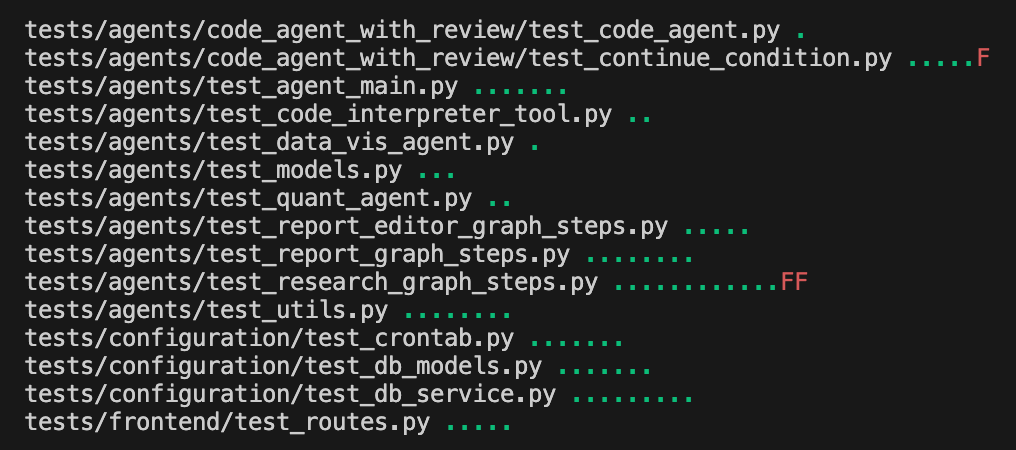
\includegraphics[width=1\textwidth]{images/test-results.png}
\caption{Test results by test file}
\end{figure}

\begin{figure}[H]
\centering
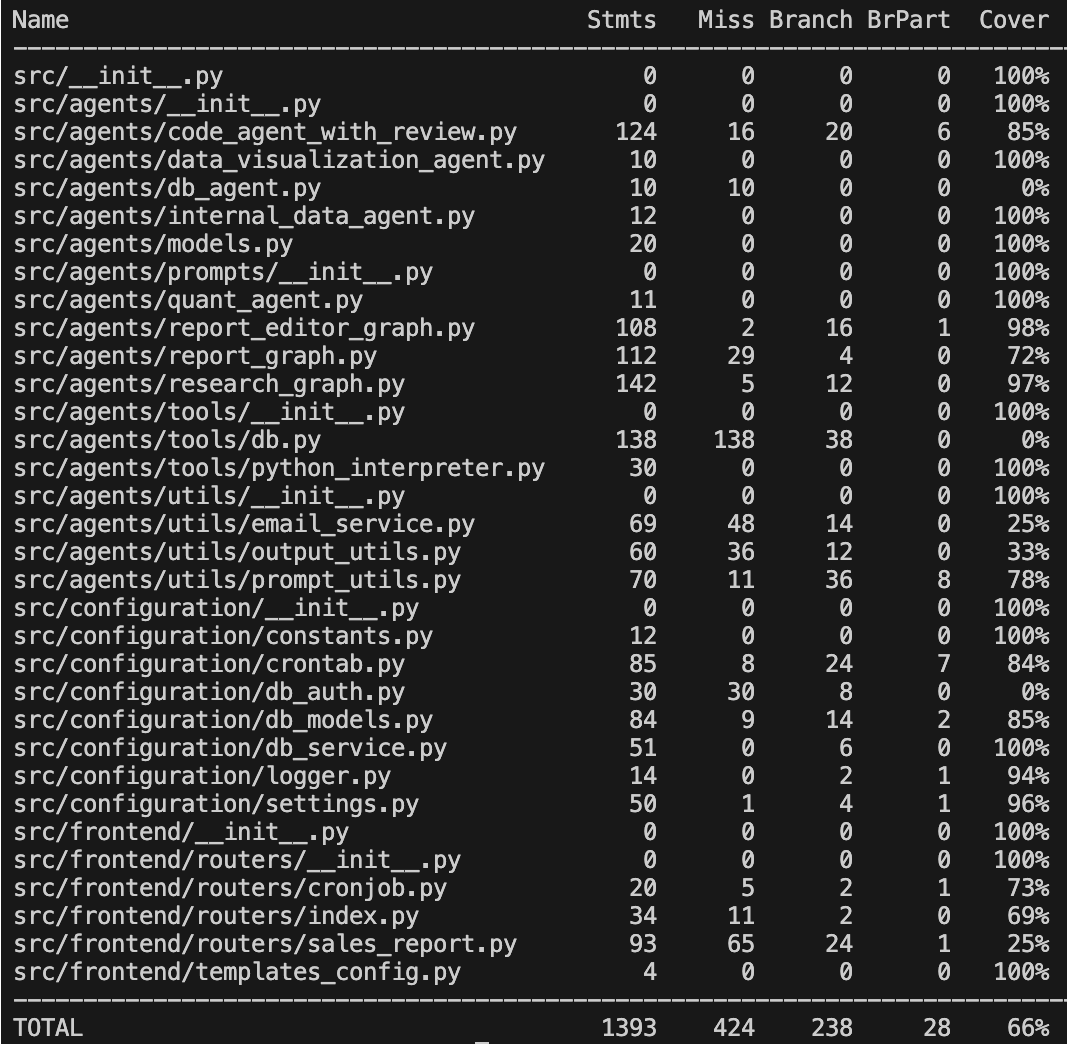
\includegraphics[width=0.5\textwidth]{images/test-coverage.png}
\caption{Test coverage output}
\end{figure}

\chapter{Generated Report --- Sample}

\end{document}